\documentclass[conference, letterpaper, 10pt]{IEEEtran}

\usepackage[utf8]{inputenc}

\title{On the security of encryption and compression composition under reflection attacks}

\author{
    Anonymized submission
}

%  \author{
%      \IEEEauthorblockN{Dimitris Karakostas}
%      \IEEEauthorblockA{University of Athens \\
%      dimit.karakostas@gmail.com}
%      \and
%      \IEEEauthorblockN{Aggelos Kiayias}
%      \IEEEauthorblockA{University of Edinburgh\\
%      akiayias@inf.ed.ac.uk}
%      \and
%      \IEEEauthorblockA{Dionysis Zindros}
%      \IEEEauthorblockA{University of Athens \\
%      dionyziz@di.uoa.gr}
%  }

\usepackage{url}
\usepackage{amsmath}
\usepackage{graphicx}
\usepackage{listings}
\usepackage{mathtools}
\usepackage{amsfonts}
% \usepackage{amsthm}
\usepackage{amssymb}
\usepackage[colorlinks=true,linkcolor=black,citecolor=black]{hyperref}

\usepackage{cite}

\DeclarePairedDelimiter{\ceil}{\lceil}{\rceil}
\let\oldemptyset\emptyset
\let\emptyset\varnothing

\newtheorem{lemma}{Lemma}

\newcommand\defeq{\stackrel{\mathclap{\normalfont\mbox{def}}}{=}}
\newcommand{\overbar}[1]{\mkern 1.5mu\overline{\mkern-1.5mu#1\mkern-1.5mu}\mkern 1.5mu}

\begin{document}

\maketitle

\begin{abstract}
When compression is composed with encryption, unexpected vulnerabilities can
arise. Such vulnerabilities have been explored in practical attacks against TLS
such as CRIME, TIME, and BREACH, even after TLS 1.3. We introduce an abstract
theoretical cryptographic model for such attacks, the \textit{adaptive
reflection security} game with the relevant security definitions. We propose a
model for \textit{compression idealness} and experimentally show that typical compression
functions expose partially ideal behavior. We then experimentally show that
typical plaintexts used in practice follow an interdependent joint distribution,
a stronger notion of dependent joint distributions. Based on these two
properties, we prove that \textit{compression-detectability} of predicates
arises, i.e. the ability to extract a predicate of the plaintext using reflection.
We then prove that all length-preserving encryption schemes are insecure when
composed with such functions. Our attack model describes two modes of attack,
one-shot and amplified. For the case of the BREACH attack, we discuss how it can
be described as an instance of our theoretical model. Motivated by the lack of
production-grade testing tools, we provide a modular scalable open-source
generic attack framework that implements compression side-channel attacks in a
robust manner. Finally, we propose a novel defense protocol, \textit{context
hiding}, that effectively eliminates the threat these attacks pose. This
protocol modifies the plaintext joint distribution in order to remove the
interdependence and mitigate the problem. We show that our method of
defense performs significantly more favourably in terms of compression rate
compared to previous techniques.
\end{abstract}

\section{Introduction}\label{sec:prev}

Compression and encryption composition has caused serious security problems
in protocols such as TLS \cite{c15} over the years.
However, the theoretical models for these classes of attacks has been limited so
far.

We believe a generalization and abstraction of the rendering process is
essential to theoretically analyzing the security of compression and rendering
functions in general. Furthermore, generalized rendering and compression
functions help better consider specific attacks as realistic instances of the
model. Such examples are BREACH \cite{c3}, TIME \cite{c2}, and CRIME \cite{c1}, which are expressed as
instances of compression side-channel attacks in the context of real web
services and the rendering of web pages.

\subsection{A high-level overview}\label{subsec:example}
Our work is motivated by the threat compression side-channel attacks pose
against real-world systems. So far little attention has been drawn to these
attacks, primarily due to the complexity and the lack of production code tools
that allow for an easy, robust execution. However, these attacks potentially
allow for full plaintext recovery, as will be highlighted in this section's
example.

Consider the communication between a user that browses the Internet and a server
that hosts a website. This website might be a social network, e-banking, mail
provider or a similar service that handles sensitive private data. When the
server receives a request for a web page it collects all needed data, generates
the HTML code that will be displayed by the user's browser and sends a network
response containing this code along with other resources such as images and
libraries. All response data is encrypted under TLS, which ensures privacy and
integrity for the communication between the user and the server.

There also exists an adversary that aims to break this communication's security.
This adversary tries to decrypt the communication between
the user and the server and reveal information about the private data that is
exchanged. In order to achieve this, the adversary should fulfill certain
requirements.

Firstly, the adversary is able to handle the user's network traffic. That way he
is able to collect and analyze the network packets of the encrypted
communication with the server. He is also able to inject code in third-party
non-encrypted HTTP responses.

Secondly, he should be able to issue any number of malicious requests using the
user's cookies. This can be achieved by forcing the user's browser to run a
piece of code, such as a Javascript script. This script can either be hosted on
an adversary-controlled website or injected in plain HTTP responses the user
receives from third websites. This script is executed when loaded in the user's
browser and is able to issue requests to any URL crafted by the adversary.
Figure \ref{fig:attack_model} elaborates further on this attack mode.

Thirdly, the web service that is under attack should allow the adversary to
inject data in the encrypted response plaintext. This data takes the form of a
specially crafted reflection string which can be added for example by using a
HTTP GET parameter whose value is included in the HTML response.

Any adversary that fulfills these requirements can issue a compression
side-channel attack against the user and the web service. The malicious requests
contain the reflection strings and the user's cookies. The response contains
both the reflection string and the user's private data. The structure of the
reflection string depends heavily on properties of the private data and will be
further explored in the following sections.

As the attack progresses the adversary collects network data containing multiple
responses and reflections. Although this data is encrypted, analysis on the
lengths of different response packets will reveal properties of the private data.
At this point the privacy of the communication between the user and the website is
compromised and the adversary has broken the security of TLS.

    \begin{figure}[thpb]
        \centering
            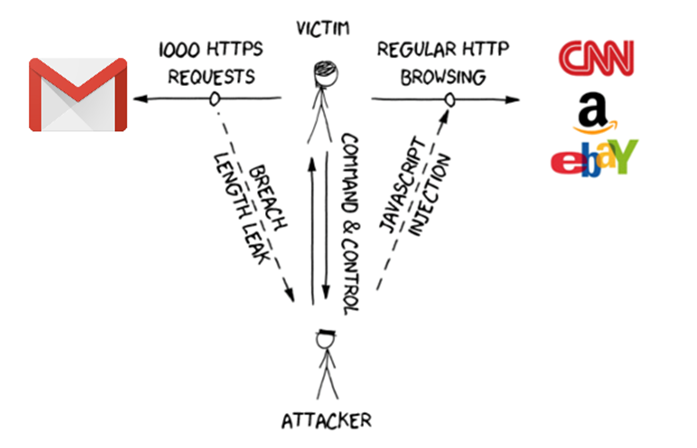
\includegraphics[width=0.48\textwidth]{attack_model.png}
        \caption{The attack model}
        \label{fig:attack_model}
    \end{figure}

\subsection{A motivating example}\label{subsec:terms}
We now describe a concrete example of the website in the previously described
attack to illustrate the various terms we use in the rest of this paper.  The
terms that need be explained include the \textit{rendering function} $f$,
\textit{rendered message} $m$, \textit{secret} $s$, \textit{noise} $v$,
\textit{reflection} $r$ and the distributions $\mathcal{M}$ of secrets and
$\mathcal{V}$ of noise.

In this case, the target of the attack is the website found in the URL
\textit{mail.example.com}. The victim is the user that is logged in this mail
service and whose cookies the adversary uses in his requests.

The web page that the adversary exploits is
\textit{mail.example.com/search?query=attack}. This website provides a HTTP GET
parameter called \textit{query} and the adversary uses the reflection string
\textit{attack}. The HTML response is included below:

\begin{lstlisting}[basicstyle=\small\ttfamily]
<div>
    <p>You searched for: attack</p>
    <p>No results found.</p>
</div>
<div>
    Your inbox:
    <ul>
    <li>[Bank] Routing number: 123</li>
    </ul>
</div>
<div>
    <p>Current Time: 12:40:00</p>
</div>
\end{lstlisting}

The server's HTML generator is an instance of the \textit{rendering function}
$f$. This function implements the rendering of the HTML code based on
blueprints.

The output of $f$ is the \textit{rendered message} $m$. This is the generated
HTML response code that contains response data and is rendered by the user's
browser.

The HTML response contains multiple data elements. A data element can be a
\textit{secret}, \textit{noise}, \textit{static}, or a \textit{reflection}.

A \textit{secret} $s$ is any part of the response that the application wishes to
remain private. The adversary wishes to learn information about $s$. Examples of
secrets in an HTML response include private messages, email contents, financial
data, and web security elements like CSRF tokens \cite{c16}. A secret's alphabet
is generally printable text characters. In our example, the strings "Bank",
which is an email topic, and "Routing number: 123", which is the email body, are
both secrets.

A \textit{reflection} $r$ is a component crafted by the attacker and can be
adaptively transformed as the attack progresses. In our example, the HTTP GET
value "attack" of the parameter "query" is used as a reflection. This string is
included in the response in the message "You searched for: attack". This serves
as an information message for the user and reflects in every search request the
value of the GET parameter "query".

The \textit{noise} $v$ is a value that changes in every request regardless of
the requested content. Examples of noise include timestamps and ads. The noise
follows a random distribution and its alphabet consists of printable characters.
In our example, the string "12:40:00" is noise.

\textit{Static} is any content that remains unchanged across requests. Typical
examples of static data are HTML $<$div$>$ tags and CSS code. Static content is
predictable and thus irrelevant in the attack. Strings like "div", "ul", "Your
inbox:" are considered static in our example.

Secrets and reflections are chosen from the distribution $\mathcal{M}$.
$\mathcal{M}$ in our example contains all routing numbers and 4-letter strings
like "Bank".

Finally, each noise element is chosen from the distribution $\mathcal{V}$. In
our example, $\mathcal{V}$ contains all 24hr timestamps. In every request, a new
noise element is chosen from $\mathcal{V}$. In this case it is "12:40:00".

The compression function $\textrm{Com}$ is the compression algorithm used on the
HTML response plaintext. In our example, this algorithm is DEFLATE, the most
common compression algorithm in the web. The composition of $\textrm{Com}$ and
the rendering function $f$ is the encoding function $\mathcal{K}$.

The encryption function $\textrm{Enc}$ is the encryption algorithm used by the
web server during the communication. The most commonly used symmetric encryption
algorithm today is AES. We use the function $\mathcal{E}$ to describe the
composition of $\textrm{Enc}$ and $\textrm{Com}$.

The input of $\mathcal{E}$ is the message $m$ and its output is ciphertext $c$.
This ciphertext is included in the network response packets and is sniffed by
the adversary over-the-wire.

The generation of $m$, its compression and encryption and the transmission over
the network of $c$, as well as the sniffing ability of the adversary, constitute
the reflection oracle that will further described in following sections.

The adversary issues the attack in stages. In each stage he creates a pool of
reflections and makes malicious requests for each reflection in the pool. An
attack stage ends when the adversary has successfully decrypted a single
character in the secret. He then adaptively changes the reflection pool, based
on the newly stolen character, and continues similarly with the next stage.

In some cases, the adversary aims at finding a property of the secret rather
than the secret itself. This property is $g(s)$ and the guess of the adversary
is $y$. When $g(s) = y$ the adversary has successfully recognized the property
$g$ of secret $s$. Finally, a special case of $g$ is a predicate $Q$.

\subsection{Contributions}
Our contributions are as follows.

First we introduce a novel model for discussing compression and encryption
composition attacks, the \textit{adaptive reflection game}, with an accompanying
security definition. This model is quite general in that it does not describe
specific instances of the rendering function $f$ or the compression function
$\textrm{Com}$. Furthermore, it allows for general distributions of secret $\mathcal{M}$
and distributions of noise $\mathcal{V}$ which can affect the rendering. Section
\ref{sec:refsec} contains the definition of this model.

We wish to prove that all encryption functions are insecure when composed with
compression. In order to make this proof, we build a series of required
assumptions.

We define \textit{interdependence}, a property that characterizes dependent
random variables drawn from a joint distribution. Interdependence is an
important notion when exploring the effects of the reflection when compressed
with a secret. We introduce interdependence in section
\ref{subsec:interdependence}.

Another property of compression functions is \textit{compression idealness}. We
define idealness in theory and demonstrate how it applies on the compression
algorithms that are widely used in section \ref{subsec:com_idealness}.

Based on the properties of compression idealness and interdependence, we prove
that predicates on the secrets can be learned by choosing adversarial
reflections. We call this property \textit{compression detectability}, which we
explore in section \ref{sec:propertycom}.

The final part of our theoretical work on the attack is to show that this
somewhat innocent property directly allows the construction of an attacker,
which we prove breaks the security of the scheme in section
\ref{sec:comattack}. We also prove that such attacks can be amplified to
achieve better confidence.

At this point we implement Rupture\footnotemark[1], a production-grade open
source framework for conducting compression and encryption composition attacks.
This generic framework provides an extensible mechanism for experimentally
testing attack techniques in a modular setting. We implement specific
compression attack instances such as BREACH. This is the first time a working
tool is provided for this class of attacks.  Based on our attack framework we
achieve significant improvements in our implementation compared to previous
attempts. We improve the complexity from linear to logarithmic in the secret
alphabet's size, we attack block ciphers in addition to stream ciphers and we
employ practical techniques for network level optimization.  Rupture is further
described in section \ref{subsec:rupture}.

Having established the attack premises, we shift our interest in defending
against such attacks. Although there are several proposed defenses, we feel that
none achieves good compression performance in real-world system terms. In this
direction, we propose \textit{context hiding}, a method that mitigates a class
of practical compression side-channel attacks like BREACH. Context hiding aims
at preventing the compression detectability of a predicate $Q$ of a secret $s$
in presense of reflection as described in section \ref{sec:defense}.

Our implementation of the context hiding defense technique is called
CTX\footnote[1]{The GitHub repositories of the Rupture and CTX projects make the
source code openly available but have been removed for anonymization purposes
and can be provided upon request.}. CTX runs at the application layer of web
services and is opt-in. It is implemented in Python and Javascript and can be
used in the common web frameworks Django, Flask and Node.js. CTX achieves
balance between security and compression performance that is unprecedented
compared to other proposed defense methods.

We experimentally show in section \ref{subsubsec:ctx_experiments} that CTX
performs well in terms of size and time overhead. Specifically, we find that the
performance penalty of CTX compared to other proposed methods, like secret
masking, is significantly lower and within accepted rates for real-world
applications.

\section{Reflection security}\label{sec:refsec}

\subsection{Adaptive reflection game}\label{subsec:refsecgame}

Let $\mathcal{PE} = (Gen, \mathcal{E}, \mathcal{D})$ be a public-key
encryption scheme, $\mathcal{A}$ be an adversary and $\mathcal{S}$ be a
simulator of $\mathcal{A}$.  The game
$\text{Game}_{\text{REF-SEC}}^{\mathcal{PE},\mathcal{A}}(\lambda,  f,
\mathcal{V}, g, \mathcal{M})$ is parameterized with a rendering function $f(\cdot, \cdot,
\cdot)$, a noise distribution $\mathcal{V}$, the security parameter $\lambda$,
some function $g$ of the plaintext vector, and a distribution of secrets $\mathcal{M}_\omega$
such that for all $\omega$ and for all secrets $s$ that exist in
$\mathcal{M}_\omega$ it holds that $|s| = \lambda$. We
require that the rendering function $f$ is polynomially computable and
reversible. Notice that the distribution of secrets is parameterized with the
history of execution $\omega$.

The challenger produces a $\lambda$-bit key $(pk, sk) \leftarrow
Gen(\lambda)$. The adversary is given $pk$, $\mathcal{V}$, $g$, $f$ and
$\mathcal{M}$.
Setting $\omega = ()$, the empty vector, the challenger initially chooses
a secret $s_0 \leftarrow \mathcal{M}_\omega$.

The adversary is then allowed to run and make arbitrary calls to a reflection
oracle, which responds potentially differently to every round $i$. The oracle
is parameterized by $s_i$, the secret unknown to the
adversary.  For the reflection oracle call, the adversary chooses a reflection
string $r$ and sends it to the oracle. The oracle produces a noise string
$v \leftarrow \mathcal{V}$ and computes $m_i = f(s_i, r, v)$. Subsequently
$m_i$ is encrypted as $c_i = \mathcal{E}_\kappa(m_i)$, and $c_i$ is sent back
to the adversary. Once $m_i$ is computed, the history vector $\omega$ is updated
with the rendered message as $\omega = \omega || m_i$ where $||$ denotes the
uniquely decodable concatenation of strings, and the next secret $s_{i+1}
\leftarrow \mathcal{M}_\omega$ is chosen. Note that, because the rendering
function $f$ is reversible, the history vector $\omega$ can be used to deduce
the history of all secrets, reflections and noises.

When the adversary decides to complete the game, they output a guess $y$. The
adversary is successful if $g(\psi) = y$, where $\psi$ is the sequence
of all secrets sampled by the reflection oracle during the course of the game.

Formally, let the public key adversarial game be defined as follows:

\begin{lstlisting}[texcl,mathescape,basicstyle=\small]
def $\text{Game}_{\text{REF-SEC}}^{\mathcal{PE},\mathcal{A}}(\lambda, f, \mathcal{V}, \mathcal{M}, g)$:
    $(pk, sk) \leftarrow Gen(\lambda)$
    $\omega = ()$
    $y \leftarrow \mathcal{A}^{\text{Reflect}^{\mathcal{E}_{pk}, \mathcal{V}}}
     (\lambda, f, \mathcal{V}, \mathcal{M}, g)$
    if $y = g(\psi)$:
        return 1
    else:
        return 0
\end{lstlisting}

Where the reflection oracle provided to the adversary is as follows:

\begin{lstlisting}[texcl,mathescape,basicstyle=\small]
def $\text{Reflect}^{\mathcal{E}_{pk}, \mathcal{V}}(r)$: \textrm{(global variable
$\psi$)}
    $s \leftarrow \mathcal{M}_\omega$
    $v \leftarrow \mathcal{V}$
    $m = f(s, r, v)$
    $\omega = \omega || m$
    $\psi = \psi || s$
    $c \leftarrow \mathcal{E}_{pk}(m)$
    return $c$
\end{lstlisting}

Let the simulator game be defined as follows:

\begin{lstlisting}[texcl,mathescape,basicstyle=\small]
def $\text{Game}_{\text{REF-SIM}}^{\mathcal{PE},\mathcal{S}}(\lambda, f, \mathcal{V}, \mathcal{M}, g)$:
    $\omega = ()$
    $y \leftarrow \mathcal{A}^{\text{ReflectSim}^{\mathcal{E}_{pk}, \mathcal{V}}}
     (\lambda, f, \mathcal{V}, \mathcal{M}, g)$
    if $y = g( \psi )$:
        return 1
    else:
        return 0
\end{lstlisting}

Where the simulator reflection oracle is configured to not answer:

\begin{lstlisting}[texcl,mathescape,basicstyle=\small]
def $\text{ReflectSim}^{\mathcal{E}_{pk}, \mathcal{V}}(r)$:
    $s \leftarrow \mathcal{M}_\omega$
    $v \leftarrow \mathcal{V}$
    $m = f(s, r, v)$
    $\omega = \omega || m$
    $\psi = \psi || s$
    return $\bot$
\end{lstlisting}

\subsection{Adversarial advantage}\label{subsec:refsecadv}

Let us now define the advantage of the adversary against a simulator:
\begin{align*}
    \text{Adv}_{\mathcal{PE}, \mathcal{A}, \mathcal{S}}&(\lambda, f, \mathcal{V}, \mathcal{M}, g) &\defeq\\
    |\Pr[\text{Game}_{\text{REF-SEC}}^{\mathcal{PE},\mathcal{A}}(\lambda, f, \mathcal{V}, \mathcal{M}, g) = 1] &-\\
    \Pr[\text{Game}_{\text{REF-SIM}}^{\mathcal{PE},\mathcal{S}}(\lambda, f, \mathcal{V}, \mathcal{M}, g) = 1]| &
\end{align*}

\subsection{Adaptive reflection security}\label{subsec:adaptiverefsec}

Given a rendering function $f(\cdot, \cdot, \cdot)$ and
a noise distribution $\mathcal{V}$, a public-key encryption scheme
$\mathcal{PE}$ is \textit{reflection-secure} if:
\begin{align*}
\forall \mathcal{M}:
\forall g:
\forall PPT \mathcal{A}:
\exists PPT \mathcal{S}:\\
\text{Adv}_{\mathcal{PE}, \mathcal{A}, \mathcal{S}}(\lambda, f, \mathcal{V}, \mathcal{M}, g) = negl(\lambda)
\end{align*}

\subsection{Non-adaptive secrets}\label{subsec:refsecnonadapt}

For the rest of this paper, we assume $s$ is chosen initially, it subsequently
remains constant and that the distribution $\mathcal{M}$ is independent of
history $\omega$. This is a special case of the above game, in the sense that we
assume that $\mathcal{M}_{()}$ is a distribution of secrets which we denote
simply $\mathcal{M}$, and subsequent random choices from $\mathcal{M}_\omega$
always return the initial secret $s$.

This simplifies the game as follows:

\begin{lstlisting}[texcl,mathescape,basicstyle=\small]
def $\text{Game}_{\text{REF-SEC}}^{\mathcal{PE},\mathcal{A}}(\lambda, f, \mathcal{V}, \mathcal{M}, g)$:
    $(pk, sk) \leftarrow Gen(\lambda)$
    $s \leftarrow \mathcal{M}$
    $y \leftarrow \mathcal{A}^{\text{Reflect}^{\mathcal{E}_{pk}, \mathcal{V}}_s(r)}(\lambda, f, \mathcal{V}, \mathcal{M}, g)$
    if $y = g(s)$:
        return 1
    else:
        return 0
\end{lstlisting}

The adversary reflection oracle is also simplified:

\begin{lstlisting}[texcl,mathescape,basicstyle=\small]
def $\text{Reflect}^{\mathcal{E}_{pk}, \mathcal{V}}_s(r)$:
    $v \leftarrow \mathcal{V}$
    $m = f(s, r, v)$
    $c \leftarrow \mathcal{E}_{pk}(m)$
    return $c$
\end{lstlisting}

And the simulator does not require an oracle for its execution:

\begin{lstlisting}[texcl,mathescape,basicstyle=\small]
def $\text{Game}_{\text{REF-SIM}}^{\mathcal{PE},\mathcal{S}}(\lambda, f, \mathcal{V}, \mathcal{M}, g)$:
    $y \leftarrow \mathcal{S}(f, \mathcal{V}, \mathcal{M}, g)$
    $s \leftarrow \mathcal{M}$
    if $y = g(s)$:
        return 1
    else:
        return 0
\end{lstlisting}

The reflection game is depicted in Figure \ref{fig:refgame}:

    \begin{figure}[thpb]
        \centering
            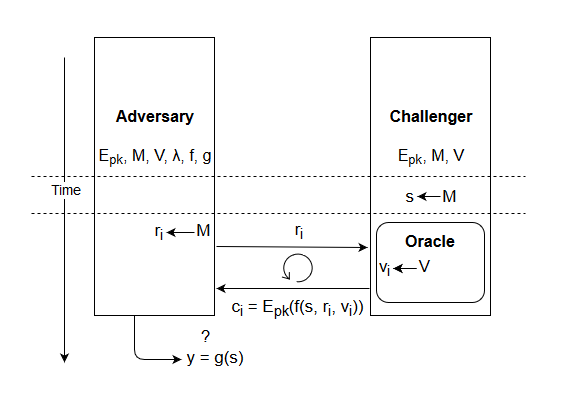
\includegraphics[width=0.48\textwidth]{reflection_game.png}
        \caption{Reflection Game}
        \label{fig:refgame}
    \end{figure}

\noindent {\bf Symmetric key version.} The above game can be modified to deal
with symmetric encryption. For this, the choice of key is changed to be limited
to a secret key instead of a public and private key pair. The adversary is not
given access to any key material.  Instead, the adversary is given access to an
encryption oracle which encrypts a given message using the secret key and
returns the respective ciphertext, in addition to the existing reflection
oracle. Both oracles can be called an arbitrary number of times by the
challenger.

In the following proofs, we will assume that the game is played symmetrically.
As the attack does not pertain to the key exchange mechanism, all theorems can
be directly translated between the two versions of the game.

\section{The security of compression}\label{sec:comsec}

\subsection{The interdependence assumption}\label{subsec:interdependence}

Let $\bar{\mathcal{M}}$ be a joint distribution from which the random variables
$(s, r)$ are drawn. We say that $s$ and $r$ are interdependent when there exist
$s_1, r_1$ and $s_2, r_2$ in the support of $\bar{\mathcal{M}}$ with $s_1 \neq
s_2$ such that:

\begin{align*}
    \Pr[(s, r) = (s_1, r_1)] &< \Pr[(s, r) = (s_1, r_2)]
\land\\
    \Pr[(s, r) = (s_2, r_1)] &> \Pr[(s, r) = (s_2, r_2)]
\end{align*}

Where the pair $(s, r)$ is drawn from the joint distribution
$\bar{\mathcal{M}}$.

It is clear that when two random variables $s$ and $r$ exhibit interdependence,
they must necessarily be dependent random variables. To see that
interdependence is a stronger version of dependence, observe that in the case
of dependence, the probability for some $s = s_1$ conditioned on $r = r_1$ is
necessarily different from the probability for some $s = s_2$ conditioned on $r
= r_2$. In interdependence, it can be seen that we additionally require the
event $s = s_1$ which was less probable than the event $s = s_2$ under the
condition $r = r_1$ to become more probable than $s = s_2$ under the condition
$r = r_2$.

We observe that commonly compressed texts such as HTML content exhibit
interdependence almost everywhere. To be more precise, if we sample, for
example, digrams (two-letter sequences) in HTML content of popular websites and
treat this two-letter sequence $\phi = (s, r)$ of the two characters $s$ and
$r$ as a random variable $\phi$, we notice that $s$ and $r$ are dependent
variables and in fact interdependent. Similarly when sampling two-word sequences
$\phi = (s, r)$ of the two words $s$ and $r$ from English literature, then $s$
and $r$ are interdependent. The same occurs for digrams in English. This
straightforward fact is supported by extensive statistical analyses in the
scientific literature such as \cite{c18}.

While the interdependence assumption is a general notion observed in all common
plaintexts, it is suitable to mention here how these ideas will emerge as we
mount our attack. In a plaintext $(s, r)$ in which the attacker controls some
reflection string $r$ and wishes to obtain information about some secret string
$s$, she wishes to distinguish between the cases $s = s_1$ and $s = s_2$ of two
different secrets $s_1$ and $s_2$, i.e. between the instances $(s_1, r)$ and
$(s_2, r)$. By measuring the difference in the probability of $(s, r)$
occurring for $r = r_1$ and $r = r_2$, the attacker can distinguish which value
of $s$ is in use. If $s = s_1$, then the attacker will observe the inequality
$\Pr[(s, r) = (s_1, r_1)] < \Pr[(s, r) = (s_1, r_2)]$, but when $s = s_2$, the
attacker will observe the different inequality $\Pr[(s, r) = (s_2, r_1)] >
\Pr[(s, r) = (s_2, r_2)]$.

The necessity of the assumption that the plaintext being compressed follows an
interdependent distribution will become clear shortly, when we introduce our
definition of compression functions. This will also immediately hint at how the
attacker is able to perform these measurements of probability inequalities
indirectly by observing ciphertext lengths.

\subsection{Composing with compression}\label{subsec:comcompose}

We now shift our interest to algorithms which compose compression and
encryption. Compression is the central point in the chain of transformations on
the plaintext. Therefore, we define the composition of a compression algorithm
with a rendering function and an encryption algorithm.

The encryption scheme above is treated as a composition of a
compression and encryption algorithm:
\begin{equation*}
    \mathcal{E} = \textrm{Enc} \circ \textrm{Com}
\end{equation*}

$\textrm{Com}$ is any polynomially computable reversible function that takes an
input string and outputs a new string: $\textrm{Com}: \{0, 1\}^* \leftarrow \{0,
1\}^*$.

$\textrm{Enc}$ denotes an encryption function. We stress our important
assumption that $\textrm{Enc}$ is defined on $\{0, 1\}^*$ and not on some
fixed-length input.

The composition of the compression function $\textrm{Com}$ and the rendering function $f$
is defined:
\begin{equation*}
    \mathcal{K} = \textrm{Com} \circ f
\end{equation*}

We call $\mathcal{K}$ an editing function. For the rest of the paper, we treat
$\mathcal{K}$ as a compression function.

\subsection{Compression idealness}\label{subsec:com_idealness}

We now move on to define the notion of compression idealness.

Let $\mathcal{K}$ be a function defined on some domain and with output space
all strings $\{0, 1\}^*$, and let $\bar{\mathcal{M}}$ be a distribution whose
support is a subset of the domain of $\mathcal{K}$.  We say that $\mathcal{K}$
is an ideal compression function with respect to the distribution
$\bar{\mathcal{M}}$ when for every $w_1, w_2$ in the support of
$\bar{\mathcal{M}}$ we have:

\begin{equation*}
\Pr[w = w_1] < \Pr[w = w_2] \iff \lvert\mathcal{K}(w_1)\rvert > \lvert\mathcal{K}(w_2)\rvert
\end{equation*}

Where $w$ is a random variable drawn from $\bar{\mathcal{M}}$.

The intuitive notion behind compression idealness is that the encoding
function is somehow perfectly aware of the input distribution. It
exploits this knowledge of the input space to encode each possible
input in an ideal way – more often occurring plaintexts are compressed
better, i.e. in shorter length, than rarely occurring plaintexts.
Practical compression functions are not perfectly ideal, because the
distribution of plaintexts they try to cover is broad and ill-defined.
However, such compression functions try to learn the distribution of
the plaintext they are about to compress by observing frequencies of
occurrences and taking advantage of them.

We now turn our attention to two specific compression functions, the
LZ77 and Huffman function. These two compression functions are of
interest for two reasons. First, they are representative of the way
typical lossless compression functions work internally, by taking
advantage of letter frequencies (Huffman) or letter-sequence (LZ77)
repetitions. Second, they are the ones almost exclusively used in
practice. The DEFLATE algorithm, which is a composition of LZ77 and
Huffman, is the algorithm used in gzip, which is prevalent on the
modern web. In 2016, 98.85\% of websites that enabled compression used
some form of gzip \cite{c19}. We argue that both LZ77 and Huffman are nearly
ideal compression functions. The complexity of the Huffman and
especially the LZ77 algorithms arises from many intricate technical
details, such as, for instance, the sliding window size of LZ77. These
details make it impractical to deal with these functions in analytical
proofs. Hence, we support our idealness claims in an experimental
manner in Figure \ref{fig:huffman_idealness}. For reference, the exact definitions of DEFLATE are given in
\cite{c12}.

    \begin{figure}[thpb]
        \centering
            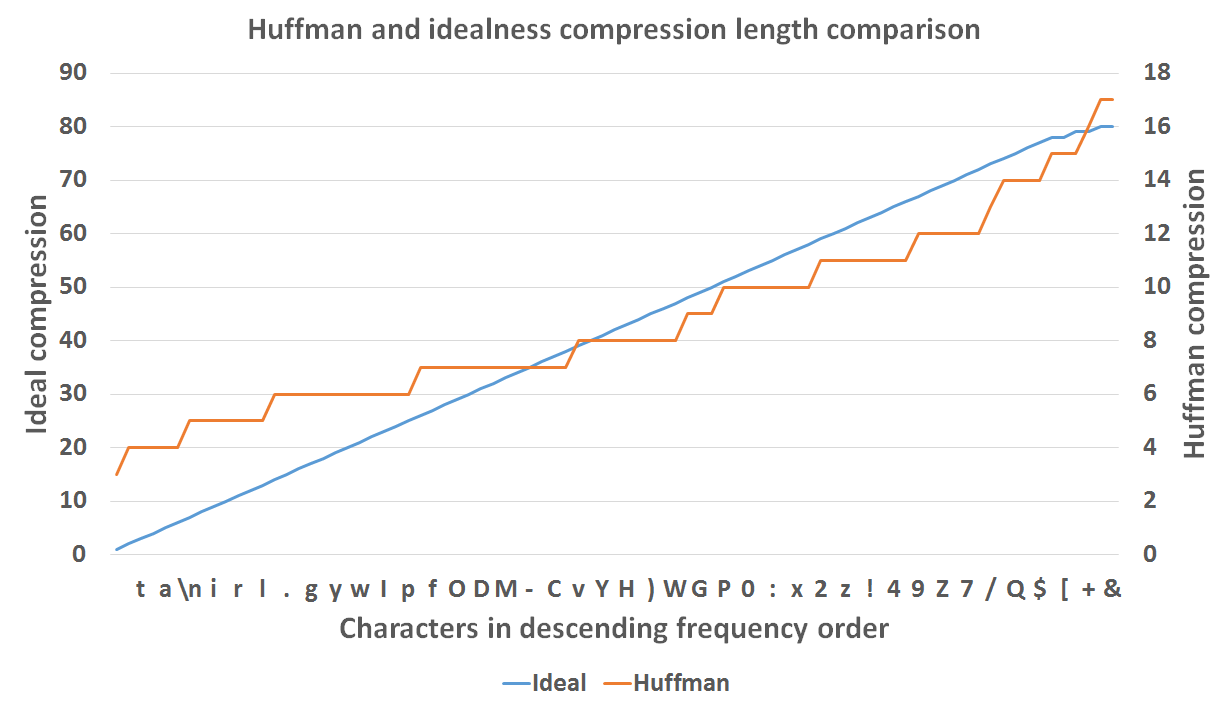
\includegraphics[width=0.48\textwidth]{idealness_experiments/huffman_idealness.png}
        \caption{Comparison between Huffman and ideal compression}
        \label{fig:huffman_idealness}
    \end{figure}

\subsection{Length monotonicity}\label{subsec:lenmonotone}

An important assumption for our attack is that the encryption function
$\textrm{Enc}$ is \textit{length monotonic}. Specifically, for any keys $k_1
k_2$ in the key generating function space and string messages $m_1, m_2$:

\begin{equation*}
\begin{split}
|m_2| > |m_1|
\Rightarrow
|\textrm{Enc}_{k_1}(m_2)| \geq |\textrm{Enc}_{k_2}(m_1)|
\end{split}
\end{equation*}

If the last inequality becomes strict, we call the encryption function
\textit{strictly length monotonic}.

A practical instance of a length monotonic encryption function is AES \cite{c8}.
Stream ciphers can be treated as strictly monotonic to the bit level.

\section{Compressibility with respect to predicates}\label{sec:propertycom}
In this section we will define compressibility with respect to predicates. We
show that all ideal compression functions that exhibit interdependence are
compression detectable by a reflection vector $\overbar{r}$ with respect to a
predicate $Q$ and a distribution $\mathcal{M}$

Let $\mathcal{M}$ be a plaintext distribution and $Q(s)$ be a predicate on the
plaintext $s$ drawn from $\mathcal{M}$. Furthermore, we require that $Q$ is not a
trivial predicate; that is, there must exist elements for which $Q$ is true and
others for which it is false.  Let us use $\mathcal{M}_Q$ to denote the
distribution $\mathcal{M}$ conditioned on the predicate $Q$.

For the specific property $Q$ and plaintext distribution $\mathcal{M}$, define:
\begin{equation*}
    \pi \defeq max(\Pr[Q(s)], 1 - \Pr[Q(s)])
\end{equation*}

Where $s$ is drawn from $\mathcal{M}$.

Let $\mathcal{V}$ be a noise distribution from which a pair of noises
$\overbar{v} = (v_1, v_2) \leftarrow \mathcal{V}^2$ is drawn.  Let $\overbar{r}
= (r_1, r_2) \in \mathcal{M}^2$ be a reflection string pair, $\mathcal{K}$ be an ideal
compression function, $f$ be a rendering function, and let $\alpha(\lambda)$ be
a non-negligible function.

We now examine how the lengths of compressing a secret $s$ rendered with
reflection strings $r_1$ and $r_2$ respectively compare.

The predicate $Q$ partitions the set $\mathcal{M}$ into two partitions
$\mathcal{M}_Q$ and $\mathcal{M}_{\lnot Q}$. We are interested in reflection
string pairs $\overbar{r} = (r_1, r_2)$ for which the comparison direction
depends on which partition $s$ belongs to.  The direction of comparison can
also depend on a noise vector $\overbar{v}$.  If $s \in \mathcal{M}_Q$, it
should compress better when reflection $r_1$ is used as compared to when $r_2$
is used. On the contrary, if $s \in \mathcal{M}_{\lnot Q}$, the opposite
direction should occur.  If this is the case for the selected reflection pair
and noise pair, we say that $Q$ compares favourably under $\overbar{r},
\overbar{v}$:

\begin{equation*}
\begin{split}
    cpr^Q_{\kappa}(s, \overbar{r}, \overbar{v})
    \defeq\\
    \begin{cases}
        |\mathcal{K}(s, r_1, v_1)| < |\mathcal{K}(s, r_2, v_2)| &\text{ if } Q(s)\\
        |\mathcal{K}(s, r_1, v_1)| > |\mathcal{K}(s, r_2, v_2)| &\text{ otherwise}
    \end{cases}
\end{split}
\end{equation*}

The reflection pair $\overbar{r}$ \textit{detects} predicate $Q$ under
compression function $\kappa$ over the secret distribution $\mathcal{M}$ and
the noise distribution $\mathcal{V}$ with advantage $\alpha$ when the
comparison is favourable for both $s_1$ drawn from $\mathcal{M}_Q$ and $s_2$
drawn from $\mathcal{M}_{\lnot Q}$. Formally, we define the predicate
$dtc_\alpha(Q, \overbar{r}, f, \textrm{Com}, \mathcal{M}, \mathcal{V})$ as follows:

\begin{align*}
    \Pr
        [cpr^Q_{\kappa}(s_1, \overbar{r}, \overbar{v}) \land
         cpr^Q_{\kappa}(s_2, \overbar{r}, \overbar{v})]
    \geq\\
    \pi + \alpha(\lambda)
\end{align*}

Where $s_1$ is drawn from $\mathcal{M}_Q$, $s_2$ is drawn from
$\mathcal{M}_{\lnot Q}$, and $v_1, v_2$ are drawn from $\mathcal{V}$.

We call $Q$ \textit{compression-detectable} with an advantage $\alpha$ if a
pair $\overbar{r} = (r_1, r_2)$ exists, such that $dtc_\alpha(Q, \overbar{r},
f, \textrm{Com}, \mathcal{M}, \mathcal{V})$ holds. Furthermore we require that such a
pair $\overbar{r}$ is polynomially computable. That is, there exists some
polynomial-time functionality $\mathcal{O}_R(\textrm{Com}, f, Q, \mathcal{M},
\mathcal{V})$ which produces an $\overbar{r}$ such that $dtc_\alpha(Q,
\overbar{r}, f, \textrm{Com}, \mathcal{M}, \mathcal{V})$ holds.

The compression-detectability property exists in all common compression
functions as long as $s$ and $r$ compress in the same context. We will now
prove the fact that all compression functions which are ideal under some
distribution $\bar{\mathcal{M}}$ exhibit compression-detectability of some
predicate $Q$.

\section{Compression attacks}\label{sec:comattack}

\subsection{One-shot attack}

\begin{lemma}[Compression attack]

Let $\textrm{Com}$ be a compression function, $\textrm{Enc}$ be a strictly length-monotonic
encryption function, $f$ be a rendering function and $Q$ be a plaintext
predicate detectable with non-negligible advantage $\alpha$ over plaintext
distribution $\mathcal{M}$ and noise distribution $\mathcal{V}$.

Then:
\begin{align*}
    \exists \alpha \text{ non-negl}:
    \forall \textrm{Enc}:
    \exists g:\\
    \exists PPT \mathcal{A}:
    \forall PPT \mathcal{S}:\\
    \text{Adv}_{\mathcal{SE}(\textrm{Enc}, \textrm{Com}), \mathcal{A}, \mathcal{S}}
    (\lambda, f, \mathcal{V}, \mathcal{M}, g) = \alpha(\lambda)
\end{align*}

\end{lemma}

\begin{IEEEproof}

Let $g$ be the boolean function $Q$ on the plaintext. Define the adversary
$\mathcal{A}$ as follows:

\begin{lstlisting}[texcl,mathescape,basicstyle=\small]
def $\mathcal{A}(Q, \mathcal{M}, y)$:
    $(r_1, r_2) \leftarrow \mathcal{O}_R(\textrm{Com}, f, Q, \mathcal{M}, \mathcal{V})$

    $l_1 = |\text{Reflect}^{\mathcal{E}_{pk}, \mathcal{V}}_s(r_1)|$
    $l_2 = |\text{Reflect}^{\mathcal{E}_{pk}, \mathcal{V}}_s(r_2)|$

    if $l_1 < l_2$:
        return True
    else:
        return False
\end{lstlisting}

Let $\mathcal{S}$ be an arbitrary simulator. Then we have:
\begin{align*}
    \Pr[\text{Game}_{\text{REF-SIM}}^{\mathcal{PE},\mathcal{S}}
        (\lambda, f, \mathcal{V}, \mathcal{M}, g) = 1] &=\\
    \Pr_{x \leftarrow \mathcal{M}, b \leftarrow \mathcal{S}(f, \mathcal{V}, \mathcal{M}, g)}
        [Q(x) = b]
\end{align*}

Letting the random variables $b$ and $x$:
\begin{align*}
    x &\leftarrow \mathcal{M}\\
    b &\leftarrow \mathcal{S}(f, \mathcal{V}, \mathcal{M}, g)
\end{align*}

Due to the independence of the simulator's output with the choice of $x$ we have:
\begin{align*}
    Pr[b = Q(x)] &=\\
    Pr[\lnot b|\lnot Q(x)]Pr[\lnot Q(x)] + Pr[b|Q(x)]Pr[Q(x)] &=\\
    Pr[\lnot b]Pr[\lnot Q(x)] + Pr[b]Pr[Q(x)] &=\\
    (1 - Pr[b])(1 - Pr[Q]) + Pr[b]Pr[Q(x)] &=\\
    1 - Pr[Q(x)] - Pr[b] + 2Pr[b]Pr[Q(x)]
\end{align*}

For a given $\Pr[Q]$, this function is monotonic in $\Pr[b]$ and therefore has
potential extrema at $\Pr[b] = 0$ or $\Pr[b] = 1$, for which cases the function
takes the values $1 - \Pr[Q(x)]$ and $\Pr[Q(x)]$ respectively. Therefore, the
maximum $\Pr[b]$ of the simulator is:
\begin{equation*}
    \Pr[Q(x) = b] = max(\Pr[Q(x)], 1 - \Pr[Q(x)]) = \pi
\end{equation*}

And therefore:
\begin{align*}
    \forall \mathcal{S}:\\
    \Pr[
        \text{Game}_{\text{REF-SIM}}^{\mathcal{PE},\mathcal{S}}
        (\lambda, f, \mathcal{V}, \mathcal{M}, g) = 1
    ]
    \leq\\
    max(Pr[Q(x)], 1 - Pr[Q(x)])
\end{align*}

From the compression detectability of Q we know that:
\begin{align*}
    \exists \alpha \text{ non-negl}:\\
    \Pr_{s_1 \leftarrow \mathcal{M}_Q,
         s_2 \leftarrow \mathcal{M}_{\lnot Q},
         \overbar{v} \leftarrow \mathcal{V}^2}
         [cpr^Q_{\kappa}(s_1, \overbar{r}, \overbar{v}) \land
          cpr^Q_{\kappa}(s_2, \overbar{r}, \overbar{v})]
    \geq\\
    \pi + \alpha(\lambda)
\end{align*}

Therefore:
\begin{align*}
    \Pr_{s_1 \leftarrow \mathcal{M}_Q,
         \overbar{v} \leftarrow \mathcal{V}^2}
         [cpr^Q_{\kappa}(s_1, \overbar{r}, \overbar{v})]
    \geq
    \pi + \alpha(\lambda) \land\\
    \Pr_{s_2 \leftarrow \mathcal{M}_{\lnot Q},
         \overbar{v} \leftarrow \mathcal{V}^2}
         [cpr^Q_{\kappa}(s_2, \overbar{r}, \overbar{v})]
    \geq
    \pi + \alpha(\lambda)
\end{align*}

And so:
\begin{align*}
    \Pr_{s \leftarrow \mathcal{M},
         \overbar{v} \leftarrow \mathcal{V}^2}
         [cpr^Q_{\kappa}(s, \overbar{r}, \overbar{v})]
    =\\
    \Pr[cpr^Q_{\kappa}(s, \overbar{r}, \overbar{v})|Q(s)]\Pr[Q(s)]
    +\\
    \Pr[cpr^Q_{\kappa}(s, \overbar{r}, \overbar{v})|\lnot Q(s)]\Pr[\lnot Q(s)]
    \geq\\
    (\pi + \alpha(\lambda))(\Pr[Q(s)] + (1 - \Pr[Q(s)))
    =\\
    \pi + \alpha(\lambda)
\end{align*}

Let us now examine the event of $\mathcal{A}$ being successful, denoted Succ,
when $cpr^Q_{\kappa}(s, \overbar{r}, \overbar{v})$. Assuming $Q(s)$:
\begin{align*}
    \Pr[|\mathcal{K}(s, r_1, v_1)| < |\mathcal{K}(s, r_2, v_2)||Q(s)]
    = \pi + \alpha(\lambda)
\end{align*}

And from the strict length monotonicity of $\textrm{Enc}$ it follows that:
\begin{align*}
    \Pr[&|\textrm{Enc}(\mathcal{K}(s, r_1, v_1))| <\\&|\textrm{Enc}(\mathcal{K}(s, r_2, v_2))||Q(s)]
        \geq \pi + \alpha(\lambda)\\
    \Rightarrow \Pr[&
        |\text{Reflect}^{\mathcal{E}_{pk}, \mathcal{V}}_s(r_1)|
        <
        |\text{Reflect}^{\mathcal{E}_{pk}, \mathcal{V}}_s(r_2)||Q(s)
    ]
        \geq \pi + \alpha(\lambda)\\
    \Rightarrow \Pr[&l_1 < l_2|Q(s)]
        \geq \pi + \alpha(\lambda)\\
    \Rightarrow \Pr[&\text{Succ}|Q(s)]
        \geq \pi + \alpha(\lambda)\\
\end{align*}

The case for $\lnot Q(s)$ is the same, but with a different inequality direction:
\begin{align*}
    \Pr[|\mathcal{K}(s, r_1, v_1)| > |\mathcal{K}(s, r_2, v_2)||\lnot Q(s)]
        \geq\\
        \pi + \alpha(\lambda)\\
    \Rightarrow \Pr[\text{Succ}|\lnot Q(s)] \geq\\
    \pi + \alpha(\lambda)\\
\end{align*}

And so the probability of success is given:
\begin{align*}
    \Pr[\text{Succ}] =\\
    \Pr[\text{Succ}|Q(s)]\Pr[Q(s)]
    +
    \Pr[\text{Succ}|\lnot Q(s)]\Pr[\lnot Q(s)] \geq\\
    \pi + \alpha(\lambda)
\end{align*}

Therefore,
\begin{align*}
    \forall PPT \mathcal{S}:
    \text{Adv}_{\mathcal{SE}(\textrm{Enc}, \textrm{Com}), \mathcal{A}, \mathcal{S}}
        (\lambda, f, \mathcal{V}, \mathcal{M}, g)
    \geq\\
    |\pi + \alpha(\lambda) - \pi| = \alpha(\lambda)
\end{align*}

Which is non-negligible.

\end{IEEEproof}

\subsection{Amplified attack}\label{subsec:amplification}

We can now amplify the attack to achieve a better probability of success by a small modification in our adversary.
The amplification is parameterized by an odd parameter $k$.

Let the amplification adversary be defined as follows:

\begin{lstlisting}[texcl,mathescape,basicstyle=\small]
def $\mathcal{A}(Q, \mathcal{M})$:
    $(r_1, r_2) \leftarrow \mathcal{O}_R(\textrm{Com}, f, Q, \mathcal{M}, \mathcal{V})$

    $low = 0$
    $high = 0$

    for $i$ = $0$ to $k$:
        $l_1 = |\text{Reflect}^{\mathcal{E}_{pk}, \mathcal{V}}_s(r_1)|$
        $l_2 = |\text{Reflect}^{\mathcal{E}_{pk}, \mathcal{V}}_s(r_2)|$

        if $l_1 < l_2$:
            $low = low + 1$
        else:
            $high = high + 1$

    if $low > high$:
        return True
    else:
        return False
\end{lstlisting}

\begin{lemma}[Amplification]

Under the assumptions of the Compression Attack Theorem against $f, \textrm{Com}$
and compression-detectable predicate $Q$ with non-negligible
detectability margin $\alpha(\lambda)$,
the amplified adversary achieves an arbitrarily large advantage
against a non-negligible subset of elements, the
\textit{amplifiable elements} distinguished by predicate $Amp$.
\begin{align*}
    \forall \textrm{Enc}:
    \exists g:\\
    \exists PPT \mathcal{A}:
    \forall PPT \mathcal{S}:\\
    \exists Amp:
    \exists B \text{ non-negl}:
    \exists C \text{ negl}:\\
    \Pr_{s \leftarrow \mathcal{M}}[Amp(s)] = B(\lambda) \land\\
    \text{Adv}_{\mathcal{SE}(\textrm{Enc}, \textrm{Com}), \mathcal{A}, \mathcal{S}_{Amp}}
    (\lambda, f, \mathcal{V}, \mathcal{M}, g) = 1 - \pi - C(k)
\end{align*}

\end{lemma}

\begin{IEEEproof}

From the fact that $Q$ is compression-detectable and from the Compression Attack Theorem, we have that:
\begin{align*}
    \Pr_{s \leftarrow \mathcal{M},
         \overbar{v} \leftarrow \mathcal{V}^2}
         [cpr^Q_{\kappa}(s, \overbar{r}, \overbar{v})]
    =\\
    \pi + \alpha(\lambda)
\end{align*}

Some elements $s \in \mathcal{M}$ allow for better compression-detectability than others under the fixed
reflection vector $\overbar{r}$. Call these elements \textit{amplifiable} and define predicate:
\begin{align*}
    Amp(s) \defeq
    \Pr_{\overbar{v} \leftarrow \mathcal{V}^2}
    [cpr^Q_{\kappa}
     (s, \overbar{r}, \overbar{v})]
    \geq
    \frac{1}{2} + \frac{\alpha(\lambda)}{2}
\end{align*}

We will now obtain a lower bound on the probability of an element being amplifiable.

Let:

% B derivation: (where \beta(\lambda) = \alpha(\lambda) / 2)
% B + (\frac{1}{2} + \alpha(\lambda)/2)(1 - B) = \pi + \alpha(\lambda)
% B + \frac{1}{2} + \alpha(\lambda)/2 - B(\frac{1}{2} + \beta(\lambda)) = \pi + \alpha(\lambda)
% \frac{1}{2} + \beta(\lambda) + B(\frac{1}{2} - \beta(\lambda)) = \pi + \alpha(\lambda)
% B(\frac{1}{2} - \beta(\lambda)) = \pi + \alpha(\lambda) - \frac{1}{2} - \beta(\lambda)
% B = (\pi + \alpha(\lambda) - \frac{1}{2} - \beta(\lambda)) / (\frac{1}{2} - \beta(\lambda))
% B = (\pi + \alpha(\lambda) - \frac{1}{2} - \frac{\alpha(\lambda)}{2}) / (\frac{1}{2} - \frac{\alpha(\lambda)}{2})
% B = (\pi - \frac{1}{2} + \frac{\alpha(\lambda)}{2}) / (\frac{1}{2} - \frac{\alpha(\lambda)}{2})
% B = \pi / (\frac{1}{2} - \frac{\alpha(\lambda)}{2}) - (\frac{1}{2} - \frac{\alpha(\lambda)}{2}) / (\frac{1}{2} - \frac{\alpha(\lambda)}{2})
% B = \pi / (\frac{1}{2} - \frac{\alpha(\lambda)}{2}) - 1
\begin{align*}
    B = \frac{\pi}{\frac{1}{2} - \frac{\alpha(\lambda)}{2}} - 1
\end{align*}

$B$ is non-negligible in $\lambda$.

Assume, for the sake of contradiction, that:
\begin{align*}
    \Pr_{s \leftarrow \mathcal{M}}
    [Amp(s)] < B
\end{align*}

Then we have:
\begin{align*}
    \Pr_{s \leftarrow \mathcal{M},
         \overbar{v} \leftarrow \mathcal{V}^2}
         [cpr^Q_{\kappa}(s, \overbar{r}, \overbar{v})]
    =\\
    \Pr_{s \leftarrow \mathcal{M},
         \overbar{v} \leftarrow \mathcal{V}^2}
         [cpr^Q_{\kappa}(s, \overbar{r}, \overbar{v})|Amp(s)]\Pr[Amp(s)]
    +\\
    \Pr_{s \leftarrow \mathcal{M},
         \overbar{v} \leftarrow \mathcal{V}^2}
         [cpr^Q_{\kappa}(s, \overbar{r}, \overbar{v})|\lnot Amp(s)]\Pr[\lnot Amp(s)]
    <\\
    B + (\frac{1}{2} + \frac{\alpha}{2})(1 - B)
\end{align*}

But then:
\begin{align*}
    B + (\frac{1}{2} + \frac{\alpha(\lambda)}{2})(1 - B) =
    \pi + \alpha(\lambda)
\end{align*}

And this contradicts the assumption that $Q$ is compression-detectable. Therefore:
\begin{align*}
    \Pr_{s \leftarrow \mathcal{M}}
    [Amp(s)] \geq B
\end{align*}

It remains to show that the advantage of the adversary can be
arbitrarily large, i.e. that for some negligible $C$ we have:
\begin{align*}
    \text{Adv}_{\mathcal{SE}(\textrm{Enc}, \textrm{Com}), \mathcal{A}, \mathcal{S}_{Amp}}
    (\lambda, f, \mathcal{V}, \mathcal{M}, g) = 1 - \pi - C
\end{align*}

Indeed, observe that the amplifying adversary performs a repeated Bernoulli
trial with $k$ repetitions and extracts a majority. Let $X$ be the number of
repetitions that are successful for the adversary. Letting $\overbar{v}_i$
be the noise chosen from $\mathcal{V}^2$ during the $i$-th round, $X$ is defined:
\begin{align*}
    X \defeq |\{ i: cpr^Q_{\kappa}(s, \overbar{r}, \overbar{v}_i) \}|
\end{align*}

$X$ follows the binomial distribution, and therefore its expected value is:
\begin{align*}
    E[X] = \frac{k}{2} + \frac{\alpha k}{2}
\end{align*}

Let Succ denote the event of the amplified adversary succeeding. Then Succ
is equivalent to $X > \frac{k}{2}$.

Because $\alpha$ is non-negligible and due to the tail bounds of the binomial
distribution, we have:
\begin{align*}
    Pr[Succ] = 1 - C(k)
\end{align*}

Where $C$ is a negligible function.
\end{IEEEproof}

\subsection{Reflection game instances}
Having established our theoretical model, it is important to explain how
practical attacks can be described as instances of this model. For this case we
describe BREACH, CRIME, and TIME in the context of the reflection security model.

These attack share some common functionality features that we describe, before
elaborating on each one separately.

The encryption algorithm and key are included in the implementation of the TLS
protocol. In most real-world systems, the encryption algorithm is AES and the
key is typically 128 or 256 bits. In relation to the reflection game, this is
represented by the $\textrm{Enc}$ and the $Gen$ functions, whereas the AES
key used for the TLS application data is $sk$. The ciphertext $c$ is the
encrypted output of the encryption function.

The support of the distribution $\mathcal{M}$ contains all strings that consist
of a known prefix concatenated with each character in the secret's alphabet. The
secret's alphabet is in typically the digits and letters of the English alphabet.
In order to bootstrap the attack, the adversary already knows this prefix of the
secret.

The adversary issues consecutive requests, each containing a candidate string
drawn from $\mathcal{M}$ as the reflection. The secret also exists in the
support of $\mathcal{M}$ so one of the reflections is bound to match it. The
goal of the adversary is to recognize which reflection that is.

The noise distribution $\mathcal{V}$ contains strings with the same alphabet as
$\mathcal{M}$. Noise data is generally unpredictable, so the adversary issues
multiple requests per reflection candidate in order to statistically bypass the
margin of error that noise introduces in the analysis. This is a practical
example of the amplified attack described in section \ref{subsec:amplification}.
We describe how statistical methods can be used to implement this in practice in
section \ref{subsec:blockalign}.

The reflection $r$ consists of the known prefix concatenated with a single
character. In cases when $r$ matches a prefix of the secret $s$, the probability
of this prefix in $c$ will be greater than in cases of no match.
Given this interdependence between the secret and the reflection the predicate
$Q$ of the secret is compression detectable by the reflection set. The
reflection vector $\bar{r}$ contains strings $r_1, r_2, ...$, where $r_i$
consists of the known prefix concatenated with character $i$ in the secret's
alphabet.

The predicate $Q$ in this case checks whether the prefix of $s$ is equal to a
certain value. Specifically, when $Q$ is detectable, the adversary is able to
find if the length of $c$ containing the reflection $r_1$ is less than
$c$ which contains the reflection $r_2$. If that is the case, then
interdependence and compression idealness lead the adversary to conclude that
$r_1$ is a prefix of $s$, thus decrypting the character in the secret that
follows the known prefix.

\subsubsection{BREACH}
As we described in section \ref{subsec:example}, the adversary that issues the
BREACH attack fulfills some basic assumptions. He has found a vulnerable
endpoint in the web service under attack which allows him to inject a chosen
reflection in the response data along with a secret. He is also able to issue an
arbitrary amount of requests from the user's browser to said endpoint and
observe the encrypted network traffic.

The challenger, in terms of the reflection game, is the server that handles the
user's request.

The secret $s$ is a predefined data element in the response that was generated
by either a user or the service. In the original BREACH paper, $s$ is a CSRF
token.

The reflection oracle constructs the encrypted responses by concatenating the
secret, the reflection, noise and static data and rendering them with function
$f$, compressing them with compression function $\textrm{Com}$ and encrypting them with
the encryption algorithm $\textrm{Enc}$. The reflection oracle in this case is the web
application framework that implements the encryption function and the underlying
web server that contains modules for compression and encryption. The final part
of the oracle, sending the ciphertext $c_i$ to the adversary, is impemented by
the Man-in-the-Middle module that gives the adversary the ability to monitor the
user's network traffic.

The rendering function $f$ is the backend that generates the HTML response code.
The HTML contains the secret, the reflection, and the noise. All will be
compressed by the compression algorithm used by the web service, the most
commonly used being the DEFLATE algorithm. The DEFLATE algorithm is the
$\textrm{Com}$ function in terms of the reflection game.

\subsubsection{CRIME}
The CRIME attack is a similar instance of the reflection game as BREACH, but
with a few key differences.

The main difference is that CRIME targets HTTP requests instead of responses. In
this case, the challenger and the oracle exist in the user's browser. The secret
$s$ is a Cookie that is included in the request, whereas the reflection $r$ is
the same GET parameter described in BREACH. In this case, the need for
reflection exists in the requests, so the responses from the target endpoint are
ignored and they need not contain the reflection.

The rendering function $f$ is the browser's function that crafts the request
payload. The compression function $\textrm{Com}$ and encryption function
$\textrm{Enc}$ are again
the DEFLATE algorithm and the TLS protocol.

The rest of the parameters are the same as in BREACH. The adversary follows the
same strategy in order to craft the reflections $r_1$ and $r_2$, compare
different size lengths of requests that contain each one along with $s$ and
decrypt a prefix of $s$.

\subsubsection{TIME}
The TIME attack's novelty is the absence of a MitM module and the usage of a
time side-channel. In this case, the adversary does not have access to the
length, as is the case in BREACH, but the timings of the responses.

This attack measures the time until the response is complete. This time value
depends on the response length, since a longer response results in slower
network transmission.

TIME as a reflection game instance is very close to BREACH. The main difference
is found in the oracle. In TIME the last part of the oracle, sending the
ciphertext $c$ to the adversary, is implemented in the same script that issues the
requests. Also the oracle does not send $c$ to the adversary, but
rather an approximation of $\rvert c \rvert$.

\section{Rupture: An improved attack}\label{subsec:rupture}
Our contributions include the development development of a production-grade
framework for implementing this class of attacks called Rupture.
Rupture was developed as part of the work on extending the BREACH attack against
modern systems and block ciphers.

As long as a vulnerable endpoint described in \ref{sec:comattack} is found,
Rupture offers the ability to inject malicious code in any computer in the
network. This code would issue requests to the endpoint and serve as a caller of
the reflection oracle that is the endpoint.

Furthermore, it enables the traffic inspection and analysis of packet
lengths. Encrypted network packets serve as the response $c_i$ from the
reflection oracle and the length of each packet is visible on the network and
captured.

In addition, Rupture offers multiple instances of oracle $\mathcal{O}_R$, based
on various $Q$ described in \ref{subsec:parallel}, and enables the automated
computation of the reflection strings in each stage of the attack.

Finally, it amplifies the attack by issuing multiple requests per candidate
symbol in alphabet $\mathcal{\Sigma}$ in order to demonstrate better probability of
success. This is achieved by grouping requests in samplesets, where each
sampleset contains requests on a symbol in alphabet $\mathcal{\Sigma}$. Requests in a
sampleset may be constructed to enable optimization methods described in
\ref{subsec:blockalign} and \ref{subsec:parallel}.

The encrypted data pertaining to one response is a \textit{sample}.  The set of
samples collected for a particular work are a \textit{sampleset}. A work
represents the set of requests needed per candidate in the secret's alphabet.

The attack is conducted in \textit{rounds}. In each round, a decision is made
about the state of the attack and more becomes known about the secret. In a
round, either the next byte of the secret becomes known, or the known alphabet
is drilled down to a smaller set. In order to compare various different
candidate alphabets, the attack executes a series of \textit{batches} of data
collection for each round.

In each batch, several works are issued and samples are collected from each probability distribution
pertaining to a candidate alphabet, forming a sampleset. When samplesets of the
same amount of samples have been collected for all the candidate alphabets,
a batch is complete and the data is analyzed. The analysis compares the samples
of different candidates and decides which is optimal, i.e. which candidate is
contains the correct guess. This decision is made with some \textit{confidence},
is expressed in bytes. If the confidence is insufficient, an additional
batch of samplesets is collected, and the analysis is redone until the
confidence value surpases a given threshold.

Once enough batches have been collected for a decision to be made with good
confidence, the round of the attack is complete and more information about the
secret becomes known.

\subsection{Block alignment}\label{subsec:blockalign}
Block ciphers are \textit{length monotonic}, but not \textit{strictly length
monotonic}, as described in section \ref{subsec:lenmonotone}. Specifically, the
length of the encrypted text is rounded to a product of $\mu$-bits, where $\mu$
is the block size, using added padding. The same applies for stream ciphers,
whose functionality is similar to block ciphers with block size 1 byte. In this
case, plaintext length difference between two messages does not always result in
length difference between the respective encrypted ciphertext.

It is possible to bypass this problem by using block alignment. Block alignment
techniques have already been explored in the literature \cite{c14}. This method
demands issuing multiple requests to the reflection oracle while including
artificial noise in the reflection string $r$.

In each request $r_{i, c}$ for each candidate $c$ in the secret alphabet, we add
increasing artificial noise. That way, all $r_{1, c}$ for all c in candidates
will contain one character of alignment noise, $r_{2, c}$ will contain two
characters and so forth. As mentioned above, the difference in length of the
compressed plaintext for the correct candidate and an incorrect one is 1 byte.
For some alignment noise length $a \in [0, \mu)$ the reflection of the correct
candidate will be $(\delta*\mu)$ and for all incorrect candidates
$(\delta*\mu)+1$. In that case, the incorrect candidates result in one more
block over the network compared to the correct one.  This ensures that one out
of $\ceil{\mu / |r_i|}$ requests will result in a block distinction between the
alphabet candidates.

Figure \ref{fig:block_alignment} intuitively depicts the block alignment technique.

   \begin{figure}[thpb]
      \centering
          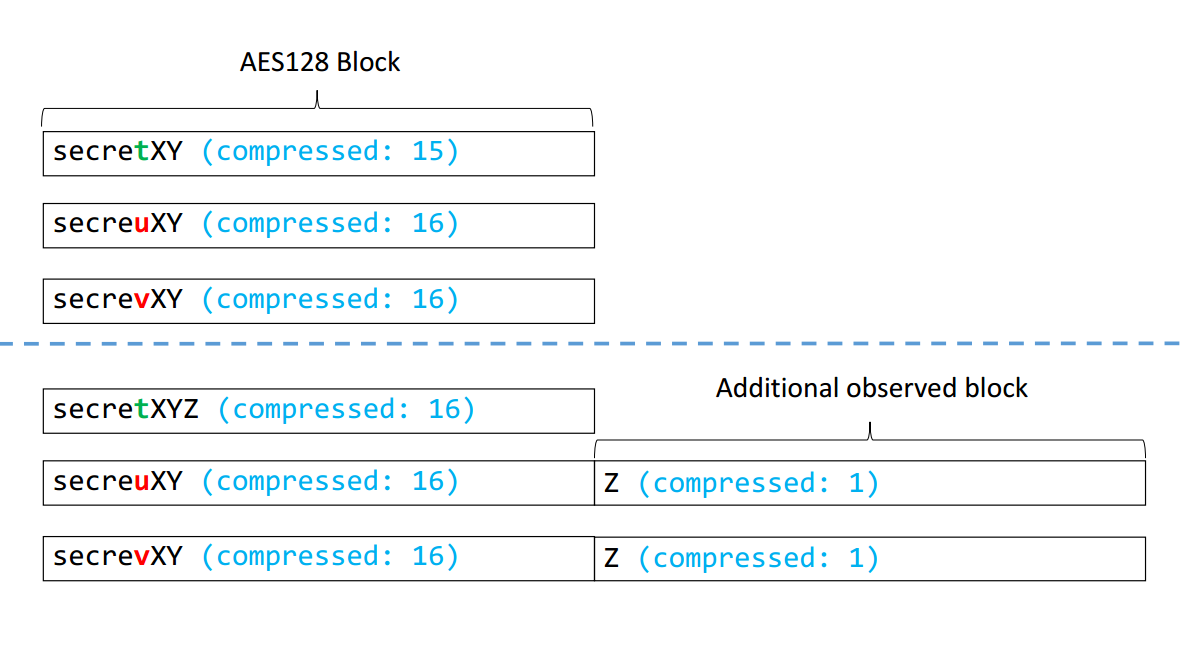
\includegraphics[width=0.48\textwidth]{block_alignment.png}
      \caption{The block alignment method}
      \label{fig:block_alignment}
   \end{figure}

\subsection{Reflection computation methods}\label{subsec:reflectionmethods}
Reflection strings $r$ should be polynomially computable, as defined in
\ref{sec:propertycom}. BREACH is
parameterized with an alphabet of ASCII symbols $\mathcal{\Sigma}$
for each character of the
secret. A successful attack should distinguish a single character of the
alphabet as the correct one through a series of requests to the reflection
oracle.

The first method of issuing requests is serial. Each request to the oracle
corresponds to a single character of the alphabet. An attack phase is completed
when requests have been issued for the entire alphabet.

In this case, $Q$ is the predicate "Given a known prefix $p_s$ of secret $s$ and
a symbol $t \in \mathcal{\Sigma}$, is $p_s || t$ a prefix of $s$?" and $\exists
s_i \in \mathcal{\Sigma}: Q(s_i)$ and $\forall s_j \in \mathcal{\Sigma} \setminus \{s_i\}:
\lnot Q(s_j)$. The complexity of the attack is $\mathcal{O}(|\mathcal{\Sigma}|)$ and
the round ends by finding a character of the secret.

The second method of attack is divide and conquer. In each phase the alphabet is
divided into two subsets $\mathcal{\Sigma}_1$ and $\mathcal{\Sigma}_2 =
\mathcal{\Sigma}
\setminus \mathcal{\Sigma}_1$, where $|\mathcal{\Sigma}_1| = |\mathcal{\Sigma}_2| =
\ceil{|\mathcal{\Sigma}| / 2}$. The reflection string for $\mathcal{\Sigma}_1$ composes of
$|\mathcal{\Sigma}_1|$ substrings divided by an annotation symbol $\beta$. Each
substring consists of the known part of the secret concatenated with a character
in $\mathcal{\Sigma}_1$. The reflection string for $\mathcal{\Sigma}_2$ is constructed
similarly. Each phase consists of one call to the reflection oracle per subset.

The predicate $Q$ in this case is "Given a known prefix $p_s$ of secret $s$, is
$p_s || t$ a
prefix of $s$, where $t \in \mathcal{\Sigma}_1$?". As long as the prefix of the
secret is \textit{compression-detectable} by each substring of the reflection,
the end of each phase marks the choice of subset $\mathcal{\Sigma}_i$ that contains
the correct alphabet symbol and the same method is applied using chosen
$\mathcal{\Sigma}_i$ as the alphabet $\mathcal{\Sigma}$. The round is complete when
$|\mathcal{\Sigma}| = 1$. Each round reduces the alphabet by half, so the complexity
of the attack with the divide and conquer method  is
$\mathcal{O}(log|\mathcal{\Sigma}|)$.

\subsection{Request parallelization}\label{subsec:parallel}
The reflection oracle is generally considered as synchronous. However, this is not
always the case, since it may be able to handle multiple parallel requests from
the adversary.

This is the case for the oracle in the practical BREACH application. In that case the reflection oracle is an endpoint
offered by a web application and the communication channel between the adversary
and the oracle is the end-to-end browser-server network channel.

Modern web servers are able to handle multiple parallel requests and
browsers can issue a certain amount of parallel requests per domain. This
functionality enables the adversary to issue multiple parallel requests per
symbol in alphabet $\mathcal{\Sigma}$ and efficiently reduce the execution time of
the attack.

\subsection{Request soup}
Previous sections demonstrated the need for multiple requests per reflection
string $r_i$. However, it is often the case that communication with the
reflection oracle given consequent analysis of each single request is time
expensive. In this case, it is preferable to issue multiple indistinguishable
requests and treat them as a set for the relative symbol.

This technique is useful in the case of the BREACH attack. In this case, communication between the browser and the
endpoint that serves as the reflection oracle is encrypted, so the analysis of
the captured packets is time expensive per request set.

A request set consists of requests for a symbol $s_i$ in alphabet
$\mathcal{\Sigma}$,
so bigger request sets result in less time delay. Length calculation per request
can then be measured as the mean length over the number of requests in the set.

This method can be combined with the methods described in \ref{subsec:parallel}
in order to utilize the parallelization and reduce the time cost of the
necessary multiple requests.

\subsection{Rupture architecture}\label{app:rupture}
Rupture consists of multiple components that collaborate in executing
compression-based attacks, such as BREACH. Each component is autonomous and
communicates with the rest over the network.

\subsubsection{Client}

The client component is a Javascript code that issues requests towards a chosen
endpoint. This endpoint serves as the reflection oracle of the attack. The client
needs to be executed from the browser of the victim that the adversary is trying
to steal secrets from. That way, the victim's authentication cookies will be
included in the request and lead to the endpoint including secrets in the
response.

The client contains minimal logic. It connects to the real-time service through
a command-and-control channel and registers itself there. Afterwards, it waits
for work instructions by the command-and-control channel, which it executes. The
client does not take any decisions or receive data about the progress of the
attack other than the work it is requested to do. This is intentional so as
to conceal the workings of the adversary analysis mechanisms from the victim
in case the victim attempts to reverse engineer what the adversary is doing.
Furthermore, it allows the system to be upgraded without having to deploy a
new client at the victim's network, which can be a difficult process.

As a regular user is browsing the Internet, multiple clients will be
injected in insecure pages and they will run under various contexts. All of
them will register and maintain an open connection through a
command-and-control channel with the real-time service. The real-time
service will enable one of them for this victim, while keeping the others
dormant. The one enabled will then receive work instructions to perform the
required requests. If the enabled client dies for whatever reason, such as a
closed tab, one of the rest of the clients will be waken up to take over the
attack.

\subsubsection{Injector}

The injector component is responsible for injecting code to the victim's
computer for execution. The injection is performed by ARP spoofing the local
network and forwarding all traffic in a Man-in-the-Middle manner. Since all HTTP
responses are infected, this provides for greatly increased robustness.

The injector component needs to run on the victim network and as such is
light-weight and stateless. It can easily be deployed on a small machine and
used for massive attacks. Multiple injectors can be deployed to different
networks, all controlled by the same central command-and-control channel.

\subsubsection{Realtime}

The realtime service is a service which awaits for work requests by clients. It
can handle multiple targets and victims. It receives command-and-control
connections from various clients which can live on different networks,
orchestrates them, and tells them which ones will remain dormant and which ones
will receive work, enabling one client per victim.

It maintains open web socket command-and-control connections with clients and
connects to the backend service, facilitating the communication between the two.

\subsubsection{Sniffer}

The sniffer component is responsible for collecting data directly from the
victim's network. As the client issues chosen plaintext requests, the sniffer
collects the respective ciphertext requests and ciphertext responses as they
travel on the network. These encrypted data are then transmitted to the backend
for further analysis and decryption.

The sniffer component has access to the victim's network traffic and
keeps track of the encrypted communication between the victim and the endpoint.
The length of the packets is unencrypted, so the sniffer is able to collenct and
report the observations on the network to the backend component.

The sniffer exposes an HTTP API which is utilized by the backend for controlling
when sniffing starts, when it is completed, and to retrieve the data that was
sniffed.

\subsubsection{Backend}

The backend component is a Python code that controls the attack execution. It
initializes the attack and calculates the initial request sets that should be
collected. It is responsible for strategic decision taking, statistical
analysis of samples collected, adaptively advancing the attack, and storing
persistent data about the attacks in progress for future analysis.

It communicates with the realtime component in order to guide the client as to
what requests need to be made at each stage of the attack. Meanwhile, it orders
the sniffer to listen and report network traffic, which is collected and stored
at the end of each phase of the attack. At each round, the backend analyzes the
sniffer reports and calculates the probability of success for the attack. At the
end of each round, property $Q$, which depends on the method of attack described
in \ref{subsec:reflectionmethods}, is detected, until the entire secret is
calculated.

   \begin{figure}[thpb]
      \centering
      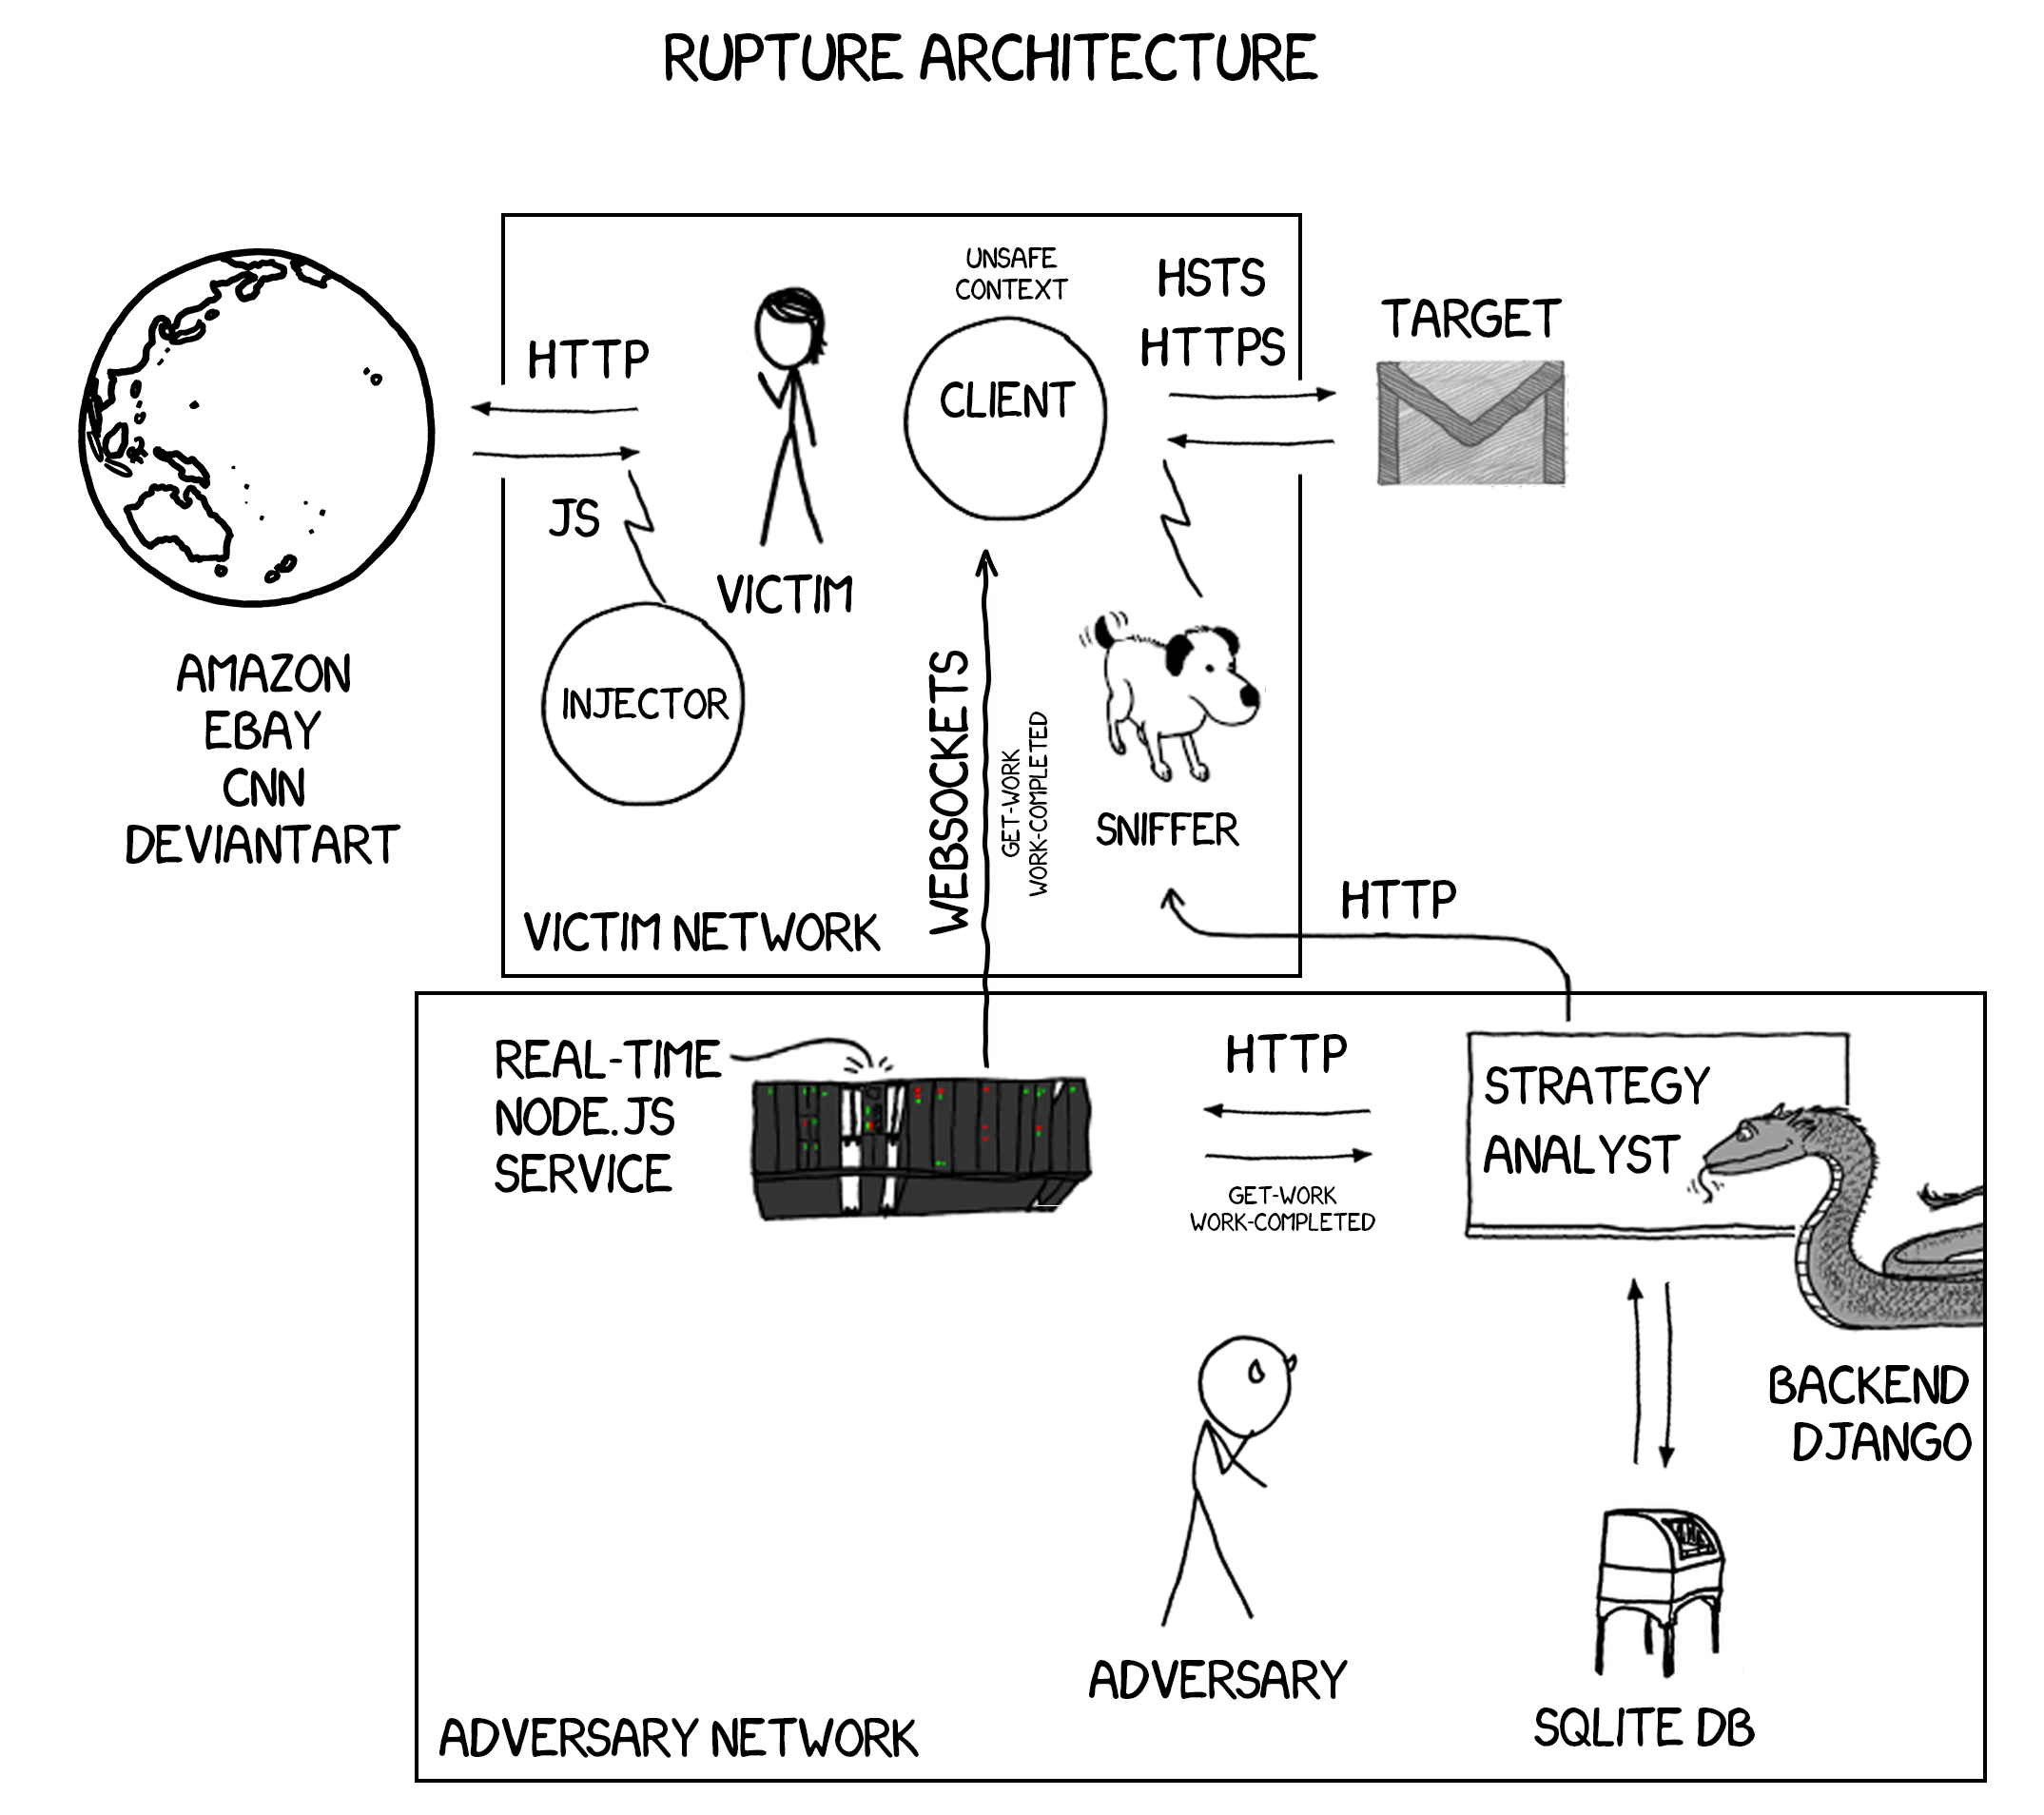
\includegraphics[width=0.48\textwidth]{architecture.png}
      \caption{Rupture Architecture}
   \end{figure}

\section{Defense: Context Hiding}\label{sec:defense}
Keeping in mind our theoretical model, we determine the key elements that make these
attacks possible.

We propose a defense, \textit{context hiding}, that mitigates a class of
practical compression side-channel attacks such as CRIME, TIME, BREACH, Rupture,
and HEIST. The full plaintext recovery these attacks perform is no longer
possible when our defense is applied.

\subsection{Attack elements from a defense perspective}
The basic problem that needs be solved is the compression detectability of
the predicate $Q$ under this class of attacks. In order to eliminate detectability,
it should be made impossible for any pair of reflections $\overbar{r}$ to detect
$Q$ under the compression function $\textrm{Com}$ and the rendering function $f$. In order to
achieve this there exist two options - either change the compression or the
rendering function.

The next step is determining what the form of the needed changes is. In order to
achieve that, we need to consider the notions that make detectability possible.
These notions are compression idealness and interdependence. The first is part
of the composition of $\textrm{Com}$ and $f$ whereas the second is part of $f$. That
said, removing either of these notions from the functions will strip the
adversary the ability to detect $Q$.

The first choice is forcing the compression function to act non-ideally in the
cases of secrets. Proposed defenses like disabling compression for annotated
secrets, or for the whole response, serve this exact idea.

The second choice is removing the interdependece between reflections and
secrets. In order to achieve that we need to decorrelate the probability of each
secret from the reflection. A method that uses this option is secret masking,
described in section \ref{subsec:masking}. Context hiding also builds on this
option and is described in the following sections.

\subsection{Context hiding properties}

Context hiding is built on the premise of separating secrets in a per-origin
manner in order to avoid cross-compression. In order to achieve this we define
what constitutes an origin and what properties same-origin secrets share. This
section describes the key components of the defense and the code implementation.

\subsubsection{Origins}
An origin is a uniquely identifiable party that generates content. A party can
be either a physical entity, like a user, or an application that provides a
service. It is important to properly identify the party that generated, or could
have generated, a piece of content. The definition of origins should reflect the
ability to generate all content that is assigned to each origin.

\subsubsection{Same-origin secrets}
Defining origins is the first step to identifying same-origin secrets. Secrets
are content pieces that are assinged to origins. Secrets that are assigned to an
origin should have been generated by the party that this origin identifies.
Also the origin's party has access to all content in this origin. This results
in a secret $a$ being insecure for all other secrets belonging in $a$'s origin.

\subsection{Context hiding functionality}
Our defense method proposes disabling cross-compression by applying a simple
substitution cipher derived from a random permutation of the plaintext alphabet.

Firstly, we identify the origins based on the output $m$ of rendering function
$f$ and store them in array $origins$. Each secret $s_i$ in $m$ is then
separated based on its origin. Each origin is uniquely identified by an integer
in range $[0, |origins|-1)$.

Secondly, we identify the alphabet for each origin. An origin's alphabet
consists of all possible characters that a secret of this origin may contain.
For each origin, we generate a random permutation of the origin's alphabet and
store it in the array $permutations$. The first element in the $permutations$
array corresponds to the first origin in the $origins$ array and so forth.

In order to secure a secret $s$ we apply a hiding function. The hiding function
\textit{hide} takes two arguments, the secret $s$ and the permutation $p$ of the
secret's origin. It applies the substitution cipher on each character in $s$ and
returns the permuted secret $s'$. The substitution cipher is implemented in the
function $Permute_p(c)$, which finds the index $i$ of character $c$ in the sorted
permutation $p$ and replaces it with the $i$-th character in $p$.

\begin{lstlisting}[texcl,mathescape,basicstyle=\small]
def hide($s, p$):
    $s' = ''$
    for $ch \in s$:
        $s' = s' || Permute_p(ch)$
    return $s'$
\end{lstlisting}

The protected secret $s'$ is annotated by the special characters
$\beta_{start}^i$, $\beta_{end}^i$ that mark the start and the end of any
substring that needs to be unpermuted.

The output $m'$ that is produced after hiding all secrets includes the
permutation array $permutations$, so that applying the reverse permutation on
all secrets is possible.

The permuted secrets in $m'$ can be retrieved using the special annotation
characters $\beta_{start}^i$ and $\beta_{end}^i$ that are unique per origin.

The initial secret $s$ can be retrieved from the protected secret $s'$
using the \textit{unhide} function. This function takes secret $s'$ and
permutation $p$ of the secret's origin and applies the reverse permutation on
$s'$, returning the unpermuted secret $s$.

\begin{lstlisting}[texcl,mathescape,basicstyle=\small]
def unhide($s', p$):
    $s = ''$
    for $ch \in s'$:
        $s = s || Unpermute_p(ch)$
    return $s$
\end{lstlisting}

\subsection{The CTX defense}\label{subsec:ctx}

\subsubsection{Implementation}
Our contributions include the development of the CTX defense. CTX is an
implementation of the context hiding method described in the previous section
for HTML web pages.

It is up to the application developer to decide which portions of the response
are sensitive and must be protected as secrets. Sensitive data does not only
include high-value secrets such as passwords and CSRF tokens, but also user data
that the developer wishes to keep private. Some examples are the bodies of email
messages in Gmail, the chat messages received or sent to a friend on Facebook,
the contents of documents and spreadsheets in Google Docs and the list of online
friends on Facebook or Google Hangouts, as they contain all the important
contacts of the victim. Practically any piece of information which is only
accessible when logged in is potentially a secret and should be CTX protected.
On the other hand, some data do not typically need compression-security
protection, e.g. static HTML portions that are accessible on a website even when
logged out.

The minimum amount of origins is one origin for the entire response, in which
case CTX is not protecting any part of the plaintext, and the maximum is one
origin per character. The latter would result in the best possible security
under CTX, although compression would be effectively disabled - possibly resulting
in poor performance. This is the case with defenses such as secret masking.

Different-origin secrets are then forced to compress separately, i.e. not
cross-compress. However, compression is achieved within each context. The
default origin alphabet is ASCII characters (0 - 128). In order to randomly
permute the secret alphabet, we use the Fisher--Yates shuffle
algorithm~\cite{c17}.

Secrets are then permuted by the server using the generated permutation of the
corresponding origin prior to TLS encryption and network transmission. Upon
arrival on the client side, the inverse permutation is applied to decode the
secret. The same permutation is applied to all secrets of the same origin. That
way, better compression is achieved intra-origin.

Each time the server issues an HTTPS response, new per-origin permutations are
generated. Compression side-channel attacks in general rely on the assumption that we can
perform multiple requests to the target website while the transmitted secret
remains the same. Since new alphabet permutations are generated per HTTPS
response, the statistical analysis performed by Rupture is no longer feasible.

\subsubsection{Experimental results}\label{subsubsec:ctx_experiments}

We have conducted several experiments to evaluate the performance of web
services protected by CTX. The results of these experiments are overwhelmingly
positive.

The CTX parameters that affect performance are basically 3: the number of
origins, the total response size in bytes, and the amount of
secrets in the response. Each parameter affects the performance differently and
will be examined thoroughly in the following sections. Our experiments focused
on each parameter separately, so the results reflect the performace under each
one independently.

In all our tests we use an HTML web page where the secrets are strings of
English literature. The tests measure the performance penalty in terms of size
overhead in the compressed response HTML. The penalty in execution time is
considered insignificant and not included when less than 10ms.

However, it should be noted that our tests are particularly strict. A typical
website response consists mainly of HTML code or libraries that usually need not
be protected. In this case, the amount of secrets in the response would not
exceed 1\% of the total response, in which case the CTX overhead as shown by our
experiments is acceptable. For example, Facebook and Gmail, which offer web
pages that are ~600KB typically need only protect approximately 0.5\% of the
response.

The first parameter, the number of origins, mainly affects the compression
performance of the secrets. The more origins are used the bigger the response,
both compressed and uncompressed, will be. This is expected, given the fact that
secrets from different origins do not cross-compress.

Our experiment covered a 650KB web page, which consists of 1\% secrets and 99\%
static data. The secrets are distributed in origins that range from 1 to 50, so
the length of a secret per origin is reduced as origins increase and the total
amount of secrets and static data remains the same. We consider 50 origins a
reasonable choice since a typical response contains data generated by multiple
users and web services.

    \begin{figure}[thpb]
        \centering
            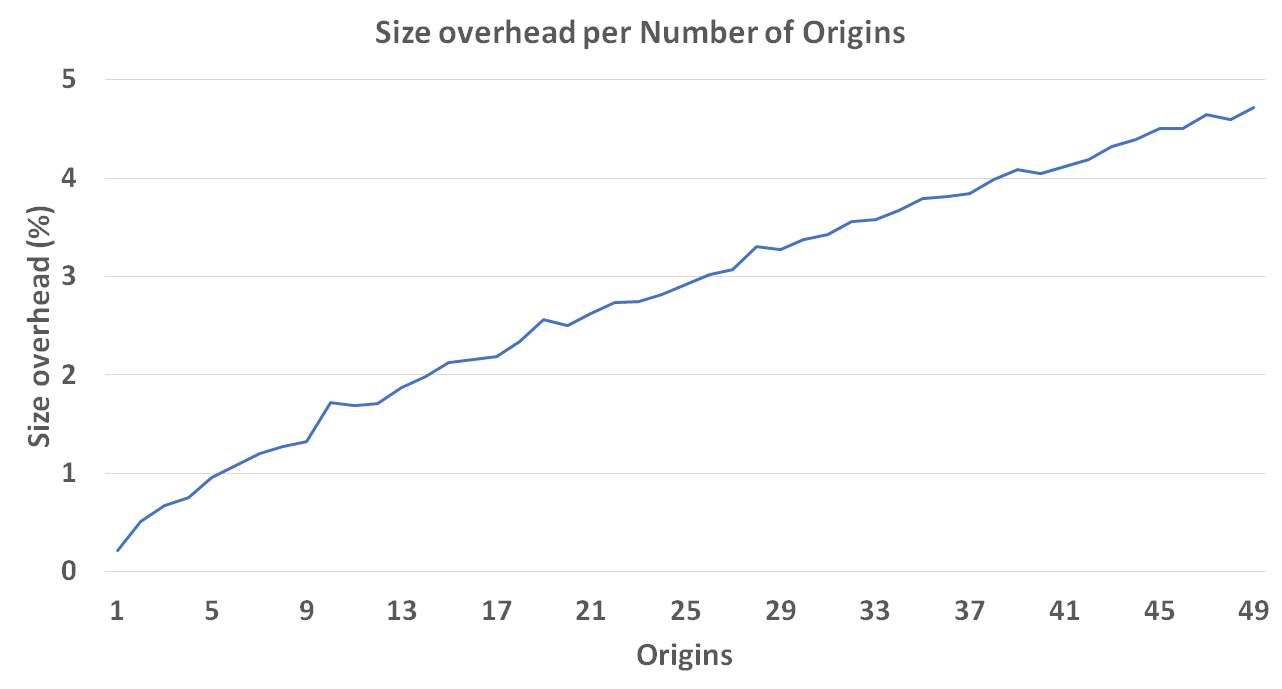
\includegraphics[width=0.48\textwidth]{experiments/origins.png}
        \caption{Origins}
        \label{fig:origin_ctx}
    \end{figure}

As Figure \ref{fig:origin_ctx} shows, the size overhead when 1 origin is used is less than 0.5\%
and about 4.7\% when 50 origins are used. This means that the compressed
response when CTX is used is expected to be 1.47x the unprotected compressed
response when 50 origins are used.

The second parameter, the total response size in bytes, affects the impact of
CTX on the compressed response.

In this case, we use 50 origins and consider 1\% of the total response to be
secret, equally distributed in all origins. The total response ranges from a
13KB to a 650KB web page.

Our experiments show that the increase in bytes that CTX adds is not
proportional to the increase of the total response size. This results in a
significant response size increase for small web pages, which becomes less
observable as the web page grows larger.

    \begin{figure}[thpb]
        \centering
            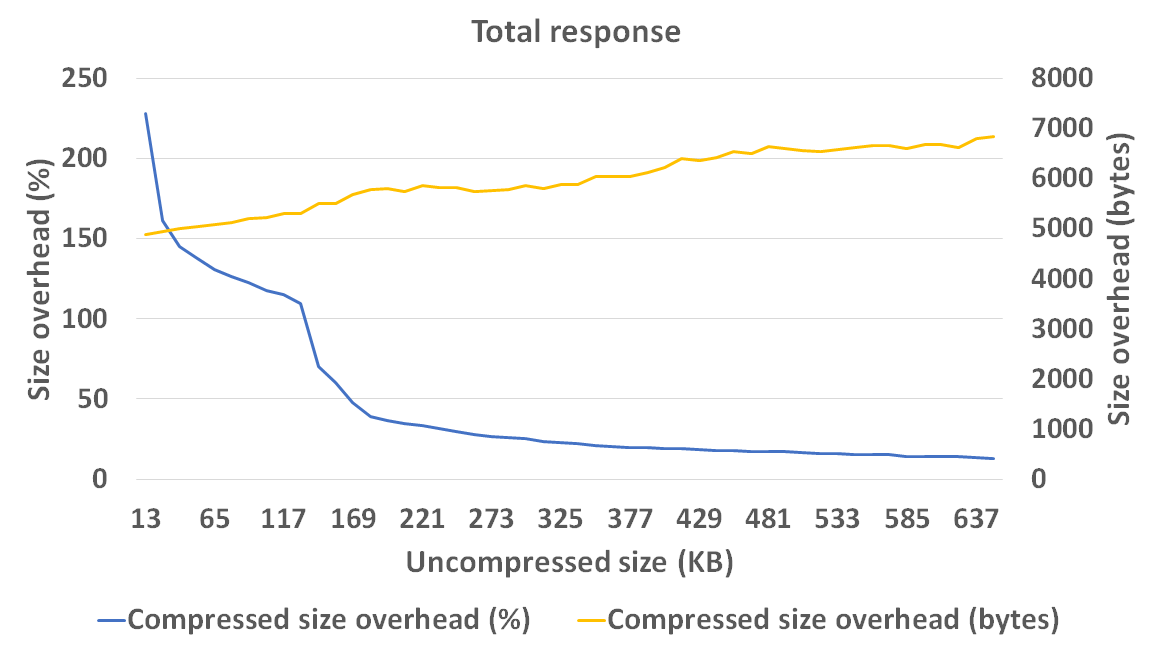
\includegraphics[width=0.48\textwidth]{experiments/total_response.png}
        \caption{Total response}
        \label{fig:total_response_ctx}
    \end{figure}

Figure \ref{fig:total_response_ctx} depicts the results of this experiment. A 13KB web page suffers a 5KB
CTX overhead, which corresponds to a 228\% increase in compressed response. On the
other hand, CTX will add only 7KB of compressed data for a 650KB web page, which
results in a 12\% increase. Disabling compression entirely would add overhead
that ranges from 500\% to 1000\% for the tested web pages.

The third parameter is the total amount of secrets in the response. In our
example we use a 650KB web page with 50 CTX origins. The secrets range from 1\%
up to 50\% of the web page, the rest being static data, and are evenly
distributed across origins.

    \begin{figure}[thpb]
        \centering
            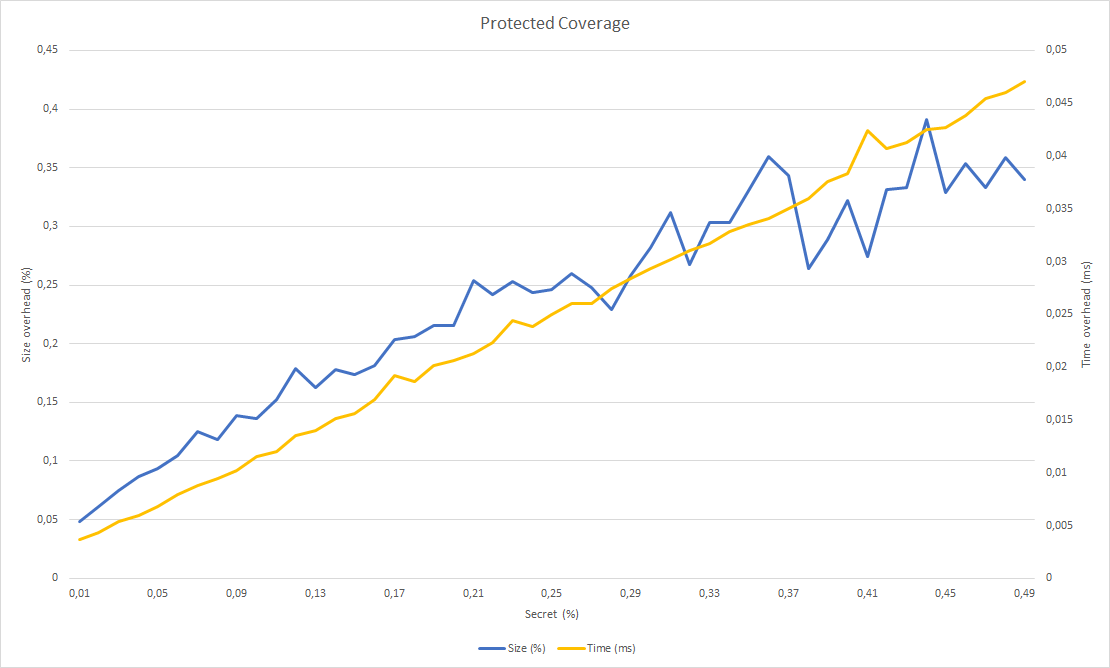
\includegraphics[width=0.48\textwidth]{experiments/response_secrets.png}
        \caption{Response secrets}
        \label{fig:response_secrets_ctx}
    \end{figure}

Figure \ref{fig:response_secrets_ctx} shows the results in this case. We find that protecting 1\% of the
tested web page results in less than 5\% size overhead, whereas protecting 50\% of
the page results in 35\%. This test also showed a noteworthy time increase in
execution time, where for 10\% secrets in the web page CTX adds 10ms of
execution time, while for 50\% it adds 47ms.

In comparison, disabling compression would again result in 976.8\% load overhead
and a network transmittion time overhead that, depending on the client's and the
server's network, may be several seconds.

\section{Related work}\label{sec:related}

\subsection{Compression attacks in literature}

The compression side-channel attack technique was first studied by Kelsey \cite{c4} in 2002.
Kelley and Tamassia\cite{c5} discuss the notion of \textit{entropy-restricted} semantic
security. However, this only models the case where two secrets compress to the same
length, making it difficult to capture practical techniques used in attacks
such as BREACH.

Alawatugoda et al. \cite{c6} introduce a model for \textit{Cookie recovery},
\textit{Random cookie indistinguishability}, and \textit{Chosen cookie indistinguishability}.
Nevertheless, their security models are limited in classes of rendering functions
that are very specific. In their models, the attacker is able to directly influence
the output of the rendering function through concatenation. More information on
rendering functions is provided in section \ref{subsec:terms}.

\subsection{Defenses}

Defense against side-channel compression attacks and especially BREACH have been
proposed in bibliography, including \cite{c3}, \cite{c5} and \cite{c6}.

\subsubsection{Disabling compression}\label{subsec:disablecom}
Compression is the basic assumption for property compressibility. Disabling
compression would break the adaptive reflection game, since it removes
the compression part of the encryption function.

However, this method is not viable, since the performance overhead should it be
applied overrules the benefits of the defense.

\subsubsection{SameSite cookies}\label{subsec:samesite}
SameSite cookies \cite{c10} is a proposed draft for enhancing web security. The
main puprose of this technique is to mitigate cross-site request forgery
attacks, although it also mitigates other kinds of cross-origin leakages.

This policy introduces a new attribute for web cookies that web servers may
opt-in. This attribute states that cookies may only be included in a
"first-party" context, i.e. in same origin requests.

However, the current BREACH application depends on cross-origin requests in
order to call the reflection oracle.
Enabling SameSite cookies would result in the elimination of this reflection
oracle of the Reflection-Security Game and the effective mitigation of the
attack.

\subsubsection{Masking secrets}\label{subsec:masking}
Masking is a method of hiding secrets' properties per request. A mask is a
bitstream equal in size with the secret. The masked text contains the result of
the XOR operation between the secret and the mask concatenated with the mask.
The secret can be obtained by applying XOR between the first and the second
half of the masked text.

A masking function is defined:

\begin{lstlisting}[texcl,mathescape,basicstyle=\small]
def masking($s_i$):
    $l = |s_i|$
    $m_i \xleftarrow{\$} \{0, 1\}^l\\$
    $s_i' = m_i \oplus s$
    return $s_i', m_i$
\end{lstlisting}

Masking can be applied on a rendered secret $s_i$ in the output $m$ of a
rendering function $f$ as:

\begin{lstlisting}[texcl,mathescape,basicstyle=\small]
def apply_masking($m_i, s_i$):
    $s_i', m_i \leftarrow masking(s_i)$
    return $Rep(m, s_i, \beta_1 s_i' \beta_2 m_i \beta_3)$
\end{lstlisting}

where $Rep(a, b, c)$ is a function that replaces all occurences of $b$ in
$a$ with $c$ and $\{\beta_1, \beta_2, \beta_3\}$ are symbols that do not
appear in $m$ before masking.

Mask removal should be applied on all masked secrets, marked by the annotation
symbols $\beta_1$, $\beta_2$, $\beta_3$, before the reversing of rendering function $f$:

\begin{lstlisting}[texcl,mathescape,basicstyle=\small]
def remove_masking($m', \beta_1, \beta_2, \beta_3$):
    return $Rep(m', \beta_1 s_i' \beta_2 m_i \beta_3, s_i' \oplus m_i)$
\end{lstlisting}

where $Rep$ is the string replacement function and $\{\beta_1, \beta_2,
\beta_3\}$ are the annotation symbols used in \texttt{apply\_masking}.

Mask $m_i$ is chosen uniformly at random, so masked secret $s_i'$ is also
random. This results in $s_i' m_i$ being indistinguishable from $r_1 r_2$ by a
compression function $\textrm{Com}$, where $r_1$, $r_2$ are random nonces chosen
uniformly at random.

Masking renews the secret $s_i'$ each time the reflection oracle is called. That
way, this method secures the secret's content against instances of the attack
that require at least two calls to the reflection oracle.

Masking doubles the size of the secret that is being protected. Furthermore,
$m_i$ and $s_i'$ are random, so the compression performance is poor. Therefore,
masking should be applied with limitation on high value secrets only, in order
to avoid significant performance drop.

Masking is a method used by Facebook \cite{c11} in order to protect CSRF tokens
against BREACH attacks.

\begin{thebibliography}{13}

\bibitem{c1} J. Rizzo and T. Duong, "The CRIME attack", Ekoparty, 2012.

\bibitem{c2} Be'ery, T. and A. Shulman, "A Perfect CRIME? Only TIME Will Tell",
Black Hat Europe 2013, 2013.

\bibitem{c3} Y. Gluck, N. Harris and A. Prado, "BREACH: Reviving the CRIME attack",
Black Hat USA, 2013.

\bibitem{c4} John Kelsey, "Compression and information leakage of plaintext", 2002.

\bibitem{c5} J. Kelley and R. Tamassia, "Secure Compression: Theory \& Practice",
2014.

\bibitem{c6} J. Alawatugoda, D. Stebila and C. Boyd, "Protecting encrypted
cookies from compression side-channel attacks", 2014.

% \bibitem{c7} D. Karakostas and D. Zindros, "Practical New Developments on
% BREACH", Black Hat Asia, 2016.

\bibitem{c8} NIST, "Announcing the ADVANCED ENCRYPTION STANDARD (AES)", 2001.

\bibitem{c9} J. Ziv and A. Lempel, "A universal algorithm for sequential data
compression", Information Theory, IEEE Transactions, vol. 23, 1977.

\bibitem{c10} M. West, "First-Party-Only Cookies", RFC Internet-Draft, 2015.

\bibitem{c11} [online] URL:
\url{https://www.facebook.com/notes/protect-the-graph/preventing-a-breach-attack/1455331811373632}
[cited November 2016]

\bibitem{c12} P. Deutsch, "DEFLATE Compressed Data Format Specification version
1.3", RFC 1951, 1996.

% \bibitem{c13} [online] URL: \url{https://ruptureit.com} [cited November 2016]

\bibitem{c14} B. Moller, T. Duong, K. Kotowicz, This POODLE Bites: Exploiting the SSL 3.0 Fallback, September 2014.

\bibitem{c15} T. Dierks, E. Rescorla, The Transport Layer Security (TLS)
Protocol Version 1.2, August 2008.

\bibitem{c16} [online] URL:
De Ryck, Philippe, et al. "Automatic and precise client-side protection against
CSRF attacks." European Symposium on Research in Computer Security. Springer
Berlin Heidelberg, 2011.

\bibitem{c17} R. Fisher, F. Yates: Statistical tables for biological,
agricultural and medical research, 1938

\bibitem{c18} M. S. Mayzner, M. E. Tresselt, Tables of Single-letter and Digram
Frequency Counts for Various Word-length and Letter-position Combinations, 1965

\bibitem{c19} [online] URL:
\url{https://w3techs.com/technologies/details/ce-gzipcompression/all/all} [cited
November 2016]

% \bibitem{c20} D. Karakostas, A. Kiayias, E. Sarafianou, D. Zindros: "CTX:
% Eliminating BREACH with Context Hiding", Black Hat Europe, 2016.

\end{thebibliography}

\end{document}
